% @Author: Moez Bouhlel

\documentclass[
a4paper,
12pt,
%twoside,
onecolumn,
titlepage,
final,
]{article} % {scrartcl}

\usepackage[utf8]{inputenc}
\usepackage[T1]{fontenc}
\usepackage[shorthands=off,english,frenchb]{babel}
%\usepackage[fixlanguage]{babelbib}
%\usepackage{polyglossia}
%\setmainlanguage{french}
%\setotherlanguages{english}

\usepackage{abstract}
\renewcommand{\abstractnamefont}{\large\bfseries}
\usepackage[toc,page]{appendix}
\renewcommand{\appendixtocname}{Annexes}

\usepackage[nottoc]{tocbibind}
\usepackage[style=alphabetic,backend=bibtex8]{biblatex}
\addbibresource{bib.bib}

\usepackage{ifxetex,ifluatex}

%\usepackage{mathspec}
\usepackage{amssymb,amsmath}

%\usepackage{xltxtra,xunicode}
%\defaultfontfeatures{Mapping=tex-text,Scale=MatchLowercase}
%\setmainfont{TeX Gyre Pagella}
%\setsansfont{FreeSans}
%\setmonofont[Mapping=tex-ansi]{Monaco}

\usepackage{color}
\usepackage[table]{xcolor}

\usepackage{lmodern}
%\usepackage{tgpagella}
\usepackage{palatino}
\usepackage{helvet}
\fontfamily{ppl}\selectfont
% \fontsize{<nominal font size>}{<baselineskip>}\selectfont

\setlength{\parskip}{8pt}
\setlength{\parindent}{0pt}
\renewcommand{\baselinestretch}{1.2}\normalsize

\usepackage{graphicx}
\graphicspath{{figures/}, {diagrams/}}
%\usepackage{svg}
\usepackage{array}
\usepackage{longtable}

\usepackage[intoc]{nomencl}
\makenomenclature

\usepackage{url}
\usepackage[% setpagesize=false, % page size defined by xetex
            % unicode=false, % unicode breaks when used with xetex
            % xetex
            ]{hyperref}
\hypersetup{breaklinks=true,
            bookmarks=true,
            pdfauthor={Moez Bouhlel; Rihab Majdoub},
            pdftitle={La Platforme CityWatch},
            pdfsubject={Mémoire de projet de fin d'études - La Platforme CityWatch},
            pdfkeywords={CityWatch, Djagora, pfe, FSS, report, internship},
            pdflang={fr},
            pdfdisplaydoctitle=true,
            colorlinks=true, % false
            citecolor=blue,
            urlcolor=blue,
            linkcolor=magenta,
            bookmarksnumbered=true,
            pdfborder={0 0 0}}

\urlstyle{same}  % don't use monospace font for urls
% Make links footnotes instead of hotlinks:
\renewcommand{\href}[2]{#2\footnote{\url{#1}}}

\usepackage{authblk}
\usepackage[acronym,toc]{glossaries}

\usepackage{minted}
%\usemintedstyle{borland}
%\usemintedstyle{tango}
\definecolor{darkBlue}{RGB}{4, 53, 98}
\definecolor{lightBlue}{RGB}{102, 153, 204}
\definecolor{lightGrey}{RGB}{245, 247, 249}
\definecolor{magenta}{RGB}{177, 0, 89}
\setminted{
    mathescape,
    linenos=true,
    numbersep=5pt,
    frame=lines,
    framesep=2mm,
    %bgcolor=lightGrey,
    %rulecolor=lightBlue,
    %framerule=1.1pt,
    tabsize=4,
}

% use upquote if available, for straight quotes in verbatim environments
\IfFileExists{upquote.sty}{\usepackage{upquote}}{}
% use microtype if available
\IfFileExists{microtype.sty}{%
\usepackage{microtype}
\UseMicrotypeSet[protrusion]{basicmath} % disable protrusion for tt fonts
}{}

\usepackage{geometry}
\geometry{
    left=3.5cm,
    right=2.5cm,
    paper=a4paper, % Change to letterpaper for US letter
    inner=2.5cm, % Inner margin
    outer=3.8cm, % Outer margin
    bindingoffset=.5cm, % Binding offset
    top=3cm, % Top margin
    bottom=2.5cm, % Bottom margin
    %showframe, % Uncomment to show how the type block is set on the page
}

%%% Custom sectioning
\usepackage{sectsty}
\allsectionsfont{\large\bfseries\scshape}

\usepackage{titlesec}
\newcommand{\hsp}{\hspace{20pt}}
% \titleformat{\chapter}[block]{\Huge\bfseries}{\thechapter \hsp {|}\hsp}{0pt}{\Huge\bfseries}
\titleformat{\section}[block]{\Large\bfseries}{\thesection \ }{0pt}{\Large \bfseries}
\titleformat{\subsection}[block]{\large\bfseries}{\thesubsection \ }{0pt}{\large \bfseries}

%%% Custom headers/footers (fancyhdr package)
\usepackage{fancyhdr}
\usepackage[bottom]{footmisc}

\usepackage{fancyvrb}
\VerbatimFootnotes

%%% Equation and float numbering
%\numberwithin{equation}{section}   % Equationnumbering: section.eq#
%\numberwithin{figure}{section}     % Figurenumbering: section.fig#
%\numberwithin{table}{section}      % Tablenumbering: section.tab#

\makeglossaries
\newglossaryentry{maths}
{
    name=mathematics,
    description={Mathematics is what mathematicians do}
}

\newacronym{RESTful}{RESTful}{Representational State Transfer}

\newacronym{RPC}{RPC}{Remote Procedure Call}

\newacronym{VCS}{VCS}{Version Control System}


\title{La Platforme CityWatch - Memoire de Projet de Fin d'Etudes}
\author{Moez Bouhlel}
\author{Rihab Majdoub}
\affil{Faculté des Sciences de Sfax, Tunisie}

\usepackage{tikz}
\usepackage{pgfplots}
\usetikzlibrary{arrows.meta}
\tikzset{%
  >={Latex[width=2mm,length=2mm]},
  base/.style = {rectangle, rounded corners, draw=black,
      minimum width=4cm, minimum height=1cm,
      text centered, font=\sffamily},
  activityStarts/.style = {base, fill=blue!30},
  startstop/.style = {base, fill=red!30},
  activityRuns/.style = {base, fill=green!30},
  process/.style = {base, minimum width=2.5cm, fill=orange!15, font=\ttfamily},
}

\usepackage{todonotes}
\newcommand{\TODO}[1]{\setlength{\marginparwidth}{3cm}\todo{#1}}
\newcommand{\HTODO}[2]{\setlength{\marginparwidth}{3cm}\colorbox{yellow}{#1}\todo{#2}}
\newcommand{\FIXME}[1]{\setlength{\marginparwidth}{3cm}\todo[backgroundcolor=red]{#1}}
\newcommand{\HFIXME}[2]{\setlength{\marginparwidth}{3cm}\colorbox{pink}{#1}\todo[backgroundcolor=red]{#2}}
\newcommand{\DONE}[1]{\setlength{\marginparwidth}{3cm}\todo[done]{#1}}
\newcommand{\HDONE}[2]{\setlength{\marginparwidth}{3cm}\colorbox{green}{#1}\todo[done,backgroundcolor=green]{#2}}

\begin{document}

\newgeometry{hmarginratio=1:1,top=0.5in,bottom=0.5in,right=0.5in,left=0.5in}
\begin{titlepage}
\begin{center}
    \begin{tabular}{p{6.2cm} c p{6.2cm}}
        \begin{center}
            \uppercase{\sffamily \bfseries
                République tunisienne \\
                ************* \\
                Ministère de l’Enseignement Supérieur et de la Recherche Scientifique
            }
        \end{center}
        &
        \raisebox{-\totalheight}{
\includegraphics[width=3.2cm]{fss-old}}
        &
        \begin{center}
            \uppercase{\sffamily \bfseries
                Université de sfax \\
                Faculté des sciences de Sfax \\
                *********** \\
                Département d'informatique et des communications
            }
        \end{center}
    \end{tabular}

    \vspace{0.2in}
    \noindent\makebox[\linewidth]{\rule{\paperwidth-2cm}{2pt}}

    \vspace{0.6in}
    \uppercase{\large \bfseries Mémoire de projet de fin d'études}\\[0.2in]

    {\bfseries Pour l'obtention du:}\\[.2in]

    \uppercase{\bf \LARGE Diplome de Licence Fondamentale en \\ Sciences de l'informatique }\\[0.5in]

    {\bfseries \large Sujet}\\[0.3in]

    % Title
    {\bfseries \Huge \color[RGB]{16,121,196}
        La Platforme CityWatch
    }\\[0.5in]

    % Submitted by
    {\bfseries \large Par} \\[0.25in]

    {\bfseries \LARGE \color[RGB]{255,90,90}
        Moez Bouhlel \\
        Rihab Majdoub
    }

    \vspace{0.4in}
    {\large \bfseries
        Soutenu le 03/06/2017 \\
        Devant le Jury
    }\\[0.2in]

    \large
    \bfseries
    \setlength{\tabcolsep}{10pt}
    \begin{tabular}{l l l}
        M. ............. & Professeur à la Faculté des Sciences Sfax & Président \\
        M. ............. & Professeur à la Faculté des Sciences Sfax & Examinateur \\
        M. Mohamed Mhiri & Professeur à la Faculté des Sciences Sfax & Encadreur univ. \\
        M. Mohamed Amri & Djagora Academy & Encadreur indus. \\
    \end{tabular}

    \vfill
    Année Universitaire 2017/2018

\end{center}
\end{titlepage}
\restoregeometry


\pagestyle{empty}
\pagenumbering{roman}

\noindent
\begin{minipage}[c][\textheight][c]{\textwidth}
\centering
\textbf{\textit{Designed to make a difference.}} \linebreak
\hfill --- \textsc{The Minus Sign}, \ \textit{A Funny Algebra Book}
\end{minipage}

\begin{otherlanguage}{french}
	\begin{abstract}
		Résumé text.
	\end{abstract}
\end{otherlanguage}

\clearpage
\begin{abstract}

The aim of the project is to design and implement a unique platform named
CityWatch for user profiling using collected data from user behaviours in the
road.

The
The aim of the project is to investigate the performance of Gismos and
to design and construct a super multi-functional Gismo.

The novel aspects of the new Gismo are described. The abstract should
perhaps be about half a page long.

The results of testing, which show the abject failure of the Gismo,
are presented.

In the conclusions proposals for rectifying the deficiences are
outlined.

\end{abstract}

\section*{Dédicaces}

Je dédie ce travail \\
A\\
Ma mére Mounira Maalej \\
A\\
L'ame de mon pére ``Mansour''\\
A\\
Mon fiançai Oussemma Walhha \\
A qui je dois mon bonheur et réussite 

En témoignage de mon immense affectation et ma grande gratitude 

Je n'oublierai jamais, ni ...

\newpage
\cleardoublepage
\section*{Remerciements}
\vspace{1.0in}
\begin{center}
 Avant de commencer à rédiger mon rapport, je tiens a adresser mes
sincères Remerciements aux personnes qui m'ont permis de mener à bien mon
travail par leurs sincères collaborations.\\
Aux termes de ce travail de recherche, nous voudrons exprimer toutes 
notre gratitude et nos reconnaissances à notre professeur et encadreur
\\[0.2in]
 \textbf{Mr.Mohamed Mhiri}
\\[0.2in]
Nous voudrons également remercier pour sa disponibilité et les
encouragements qui nous a prodigués tout au long de ce travail
de recherche.
Nous tenons également remercier vivement les membres de jury qui 
ont bien voulu accepté d'évaluer ce modeste travail qu'ils 
veillent trouver ici l'expression de nos profonds respect.\\
\TODO{Comité}
\TODO{l'équipe}
\end{center}



\clearpage
\fancypagestyle{plain}{
    \fancyhf{}
    \rfoot{\thepage}
    \renewcommand{\headrulewidth}{0pt}
    \renewcommand{\footrulewidth}{0pt}
}
\pagestyle{plain}

\setlength{\parskip}{0pt}
\hypersetup{linkcolor=black}
\setcounter{tocdepth}{3}

\tableofcontents

\clearpage
\addcontentsline{toc}{section}{Table des figures}
\listoffigures

\clearpage
\addcontentsline{toc}{section}{Liste des tableaux}
\listoftables

%\clearpage
%\renewcommand\listoflistingscaption{Liste des codes sources}
%\addcontentsline{toc}{section}{Liste des codes sources}
%\listoflistings

%\newpage

% list of abbreviations
%\nomenclature{$c$}{Speed of light in a vacuum inertial frame}
%\nomenclature{$h$}{Planck constant}

%\printnomenclature

\cleardoublepage
\setlength{\parskip}{8pt}
\renewcommand{\baselinestretch}{1.4}\normalsize
\fancyhf{}
%\fancyhead[LE,RO]{\itshape CityWatch}
\rhead{\rightmark}
\rfoot{\thepage}
\renewcommand{\headrulewidth}{1pt}
%\setlength{\headheight}{13.6pt}t
\pagestyle{fancy}
\renewcommand{\sectionmark}[1]{\markright{\thesection\ \ --\ \ #1}}
\pagenumbering{arabic}

\part{Introduction générale}
\input{introduction}
\newpage
\part{Contexte du projet}
%\section{Introduction}

%Dans le cadre de notre Licence Fondamentale en Sciences de L'informatique à
%la Faculté des Sciences de Sfax, nous avons utilisé nos connaissances pour
%réaliser un projet de fin d'études pendant un stage dans Djagora Academy.
%Ce chapitre présente une mise en contexte et une description de la problématique
%et trace les objectifs de notre projet. De tel projet consiste a réaliser une
%plateforme \FIXME{complete phrase}

Dans cette partie, nous allons présenter l'académie \textquote{Djagora Academy}
au sein duquel nous avons effectué notre stage de fin d'études et le projet
\textquote{CityWatch} que nous sommes en train de réaliser avec la communauté
de l'académie. Nous allons présenter l'objective du projet et la méthodologie de
gestion suivi pour le réaliser.

\subsection{Présentation de l'académie}

Djagora Academy est un programme de mentorat visant accompagner des étudiants
en année terminale dans la réalisation de projets d'intérêt publique dans le but
est la création des startups.

Pendant la réalisation des projets des idées des startups, les étudiants
(mentorés)  seront accompagnés par des universitaires et des industriels
(mentors) avec le soutien de plusieurs compagnies internationales, telles que
l'European Center for Leadership and Entrepreneurship Education (Eclee France,
Eclee USA), Djagora University (SénégaL), NorthStar Paradigm Education (USA),
Continental (Allemagne), Sivantos (Allemagne), Yousoft-IT (Tunisie),
Factory Campus (Tunisie).

%Considérés comme des idées de startups, les projets proposés par le comité de
%pilotage de l'Académie Djagora se substituent aux projets de fin d'études.
%La durée de réalisation d'un projet s'étale sur cinq mois. Cette période
%correspond à un cycle d'accélération de startups. Tout au long de ce cycle,
%les mentorés suivront un programme de formations généralement certifiantes.

%Mis-à-part le programme de mentorat et le cycle d'accélération de startups,
%l'Académie Djagora déclare le défi et organise une compétition tout au long
%du cycle d'accélération de startups. Nommée «Bourse des startups», cette
%compétition unique en son genre, dont l'idée est attribuée à Factory Campus,
%est une bonne opportunité pour tous les intervenants de l'Académie Djagora.
%La «Bourse des startups» vise joindre l'utile du modèle financier et des retombées
%économiques de la bourse et de l'entrepreneuriat en général à l'agréable des
%bonnes pratiques et cultures du défi, de la concurrence, du challenge et du
%leadership.

\subsection{Présentation du sujet}

Le projet consiste en la création d'un système logiciel de collecte, de
traitement, d'analyse, de fouille et de visualisation des données/informations.
Il est décomposé en deux sous systèmes. L'un se charge de la collecte. L'autre,
quant à lui, est chargé du reste; du traitement à la visualisation.
Celui, chargé de la collecte, assimile dans un premier temps à une application
mobile capable de collecter des informations d'une façon automatique en se
basant uniquement sur les capteurs intégrés aux smartphones/tablettes
(mobile sensors), soit encore de façon semi-automatique faisant appel aux
simples intéractions de l'utilisateur (utilisateur citoyen).
Le deuxième sous système assimile à une application web permettant le
traitement, l'analyse syntaxique et sémantique, la fouille des
informations/données collectées pour enfin assurer leur visualisation.

En prenant départ d'un récepteur de position, le sujet mit à résoudre les
problématiques localisations de multiple individu, la réalisation d'un module
d'itinéraire pour les véhicules vers enfin la création d'un mécanisme qui donne
la main à effectuer divers types de rapport dans une carte.

\subsection{objectifs du projet}

L'objective du projet est de former une seule plateforme qui vise une variété
des secteurs. Nous allons maximiser le nombre des types de données collectées à
fin d'avoir un ensemble des informations que nous pouvons les utiliser pour
fournir des servies de consultation et de conseil.

Ces services de consultation peuvent support des différents secteurs incluant
les secteurs de transport, de média, de santé et plusieurs autres secteurs
privés et public.

Nos services ciblent aussi les utilisateurs citoyens comme source très
important d'information. Des services d'intérêt public seront lui fournir.

\subsection{Méthode de gestion de projet utilisée}

\subsubsection{Présentation de la méthode agile SCRUM}

Scrum est une méthode de gestion de projets dans laquelle des équipes
multifonctionnelles réalisent des produits de manière itérative et incrémentale.
Tout au long de cette méthode, le développement est définit, d'une façon
incrémentale, en cycles de travail appelés Sprints. Un sprint est définit sous
la forme d'un certain nombre de tâches à réaliser au cours d'une itération.
Cette dernière ne dure jamais plus que quatre semaines (deux semaines la
plupart du temps). Les itérations s'enchainent l'une après l'autre sans
interruption. Les Sprints se terminent à une date spécifique. Ceux-ci ne
peuvent être prolongés même si le travail ne soit pas terminé. Généralement les équipes
Scrum choisissent une durée de Sprint et la maintiennent durant le projet, jusqu'à ce
qu'elles puissent encore augmenter leur productivité et utiliser alors un cycle plus court.
Au début de chaque Sprint, une équipe multifonctionnelle (environ de quatre à sept
personnes) sélectionne des tâches (exigences du client) dans une liste priorisée.
L'équipe s'accorde collectivement sur une cible constituée de ce qu'elle pense pouvoir
livrer à la fin du Sprint. Aucune nouvelle tâche n'est ajoutée durant le Sprint. Chaque
jour, l'équipe se réunit brièvement afin de contrôler sa progression et ajuster les
prochaines étapes nécessaires à la finalisation du travail restant au sein d'un Sprint. A la
fin de chaque Sprint, une revue est organisée avec les parties prenantes durant laquelle
l'équipe montre ce qu'elle a réalisé. Le feedback obtenu peut être pris en compte sur le
Sprint suivant.
Scrum insiste sur la nécessité de livrer un produit opérationnel, testé et
documenté à la fin de chaque itération.
La figure~\ref{fig:scrum-model} représente la méthode agile SCRUM. 

%\documentclass{standalone}

%\usepackage{mathpazo}
%\usepackage{tikz}

\usetikzlibrary{calc}
\usetikzlibrary{positioning}
\usetikzlibrary{shapes}

%\begin{document}

\tikzstyle{box} = [rectangle, rounded corners, draw=black, text width=10em, minimum height=3em, text centered]
\begin{figure}[htbp]
  \centering
  \footnotesize
  %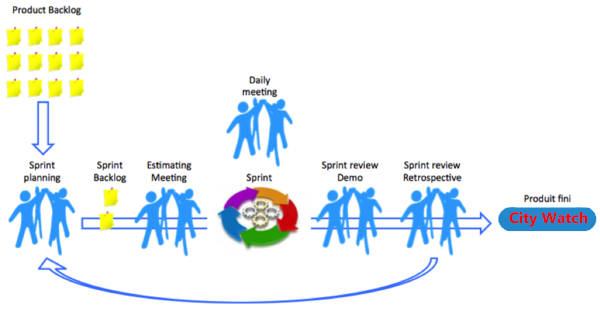
\includegraphics[width=\textwidth]{./figures/scrum-model.tex}
\begin{tikzpicture}

  \node[box]
    (sprints) {Sprints};
  \node[box, left=4em of sprints]
    (planning) {Planning \& System Architecture};
  \node[box, right=4em of sprints]
    (closure) {Closure};

  \draw[->,latex-,line width=0.1em] (5:6em) arc (5:85:6em) node[right=2em] {Wrap};
  \draw[->,latex-,line width=0.1em] (95:6em) node[left=2.5em] {Develop} arc (95:175:6em);
  \draw[->,latex-,line width=0.1em] (185:6em) arc (185:265:6em) node[left=2em] {Adjust};
  \draw[->,latex-,line width=0.1em] (275:6em) node[right=2.5em] {Review} arc (275:355:6em);

  \draw[->,latex-] (planning.west) -- +(-2em,0);
  \draw[->,-latex] (planning.east) to (sprints.west);
  \draw[->,-latex] (sprints.east) to (closure.west);
  \draw[->,-latex] (closure.east) -- +(2em,0);

\end{tikzpicture}
\caption[Méthode Scrum]{La méthode Génie Logiciel Scrum comme décrite par \textcite{Schwaber1995}.}
\captionsource{Daniel G. Siegel, Typical Development Processes of Free and Open Source Software Projects}
\label{fig:scrum-model}
\end{figure}

%\end{document}


\subsubsection{Répartition des rôles}

Chaque projet utilisant la méthode Scrum est monté autour d'une équipe auto-
organisée et multifonctionnelle : auto-organisée car il n'y a pas de chef d'équipe qui
décide les rôles de chacun, ou de la manière dont un problème est résolu, puisque ces
problématiques sont traitées par l'équipe dans son ensemble; et multifonctionnelle car
chaque membre de l'équipe forme une partie prenante dans le développement de
chaque fonctionnalité depuis l'idée jusqu'à l'implémentation finale.
Dans Scrum existe trois principaux rôles:
\begin{itemize}
 \item Le responsable produit (Product owner)
 \item Le Scrum Master
 \item le membre de l'équipe
\end{itemize}

\paragraph{Le responsable produit}

Il prend en charge de communiquer la
vision globale du produit à l'équipe. 
Il se voit représenter le client final, se met à sa place
et priorise ses besoins. Celui qui tient ce rôle est celui qui 
a le plus de visibilité, de responsabilité et d'autorité.
En effet, la méthode Scrum favorise l'auto-organisation de l'équipe.

\paragraph{Le Scrum Master}

Il joue le rôle du communiquant entre le responsable produit et
l'équipe. Il ne gère pas l'équipe, mais veille à éliminer tous les obstacles qui peuvent
empêcher l'équipe d'atteindre les objectifs fixés au cours d'un Sprint. En résumé, ce rôle
permet à l'équipe de rester créative et productive, tout en veillant à ce que les
réalisations soient visibles pour le responsable produit.

\paragraph{L'équipe}

Dans la méthode Scrum, l'équipe est responsable de la réalisation
opérationnelle des Sprints. L'équipe est généralement composée de personnes
multitâches. C'est toute l'équipe qui est responsable du résultat final de chaque sprint.
La manière dont sont exécutées les tâches est très libre mais cette liberté doit être
néanmoins cadrée par l'obligation de répondre aux objectifs du sprint.

\subsubsection{Durées estimées}

Pour montrer l'avancement durant une itération donnée, on a besoin de tracer le
Burndown Chart. Il s'agit d'un graphique simple qui montre le nombre d'heures restant
à effectuer pour finaliser le produit. 

\subsection{Justification du choix de la méthode agile SCRUM}

Aujourd'hui, La méthodes classique présente beaucoup des inconvénients 
\begin{itemize}
 \item Parfois le client a
du mal à exprimer son besoin. Une telle erreur peut s'avérer 
coûteuse d'autant la modification
de certaines fonctionnalités dans le projet n'est pas
tolérée dans la phase de développement.
 \item il est très difficile d'établir dès
le début des paramètres stricts et clairs qui répondent aux attentes du client.
\end{itemize}
Afin éviter ces problèmes, Les caractéristiques de la méthode SCRUM offre
des avantages considérables pour gérer ces problèmes.
\begin{description}
 \item [Personnel engagé] L'une des caractéristiques de SCRUM, 
 c'est que le personnel participe activement à la définition des activités et
 des horaires, de sorte que le degré d'engagement et la motivation sont plus élevés.
 \item [Meilleur vue d'ensemble du projet] Avec SCRUM, les projets 
 précédemment vus dans leur globalité et de façon homogène uniquement par
 les gestionnaires de projets sont désormais accessibles à tous les membres de
 l'équipe de livraison.
 \item [Réduction des bugs] La méthode SCRUM privilégie la qualité et la
 fonctionnalité des développements. Le nombre de bugs et
 de reprises est ainsi réduit.
 \item [Mise à jour des priorité] Au début, le client ignore toute 
 la portée de l'application, ainsi que la façon dont cela pourrait changer avec 
 le temps. Grâce à SCRUM, le client bénéficie d'une flexibilité 
 au niveau de la définition, de l'évolution des priorités et des séquences d'activités.
 \item [Qualité du produit mise en avant] La méthode SCRUM se concentre davantage 
 sur la fourniture d'un service de valeur au client plutôt que sur 
 une date limite fixée.
\end{description}

Scrum est la méthode idéale pour le cas d'une petite équipe et le fait d'avoir un grand 
projet réparti entre cette équipe et aussi il est paraît la meilleure solution pour 
répondre aux exigences du client et réduire la complexité croissante de 
certains projets.

\subsection{Conclusion}

Cette partie nous a permis de présenter le contexte général de notre projet ainsi que la
méthodologie de développement que nous allons adopter

\newpage
\part{Itérations}
\section{Itération 0}
\subsection{Présentation du contexte}
Dans le cadre de notre Licence Fondamentale en Sciences de L'informatique à 
la Faculté des Sciences de Sfax,Nous avons utilisé nos connaissances pour 
réaliser un projet de fin d'études pendant un stage dans Djagora Academy .
Ce chapitre présente une mise en contexte et une description de la problématique
et trace les objectifs de notre projet.De tel projet consiste a réaliser une
plateforme
Avant de commencer la première itération du Scrum, une période de temps à été
consacrée pour préparer ce qui est nécessaire au lancement du projet dans de bonnes
conditions. cette période est souvent nommé l’itération 0 du projet. Elle est consacrée
généralement à la recherche bibliographique, aux choix technologiques et à la mise en
place de l’environnement de développement. Outre que ces préparatifs, c’est dans cette
itération que nous définissons le Backlog de la Plateforme, ainsi que le nombre
d’itérations nécessaires et la durée de l’itération. Il s’agit aussi d’une période de
formation pour les membres de l’équipe sur tous les environnements et les technologie à
utiliser au cours du montage du produit.
\subsection{Présentation de l'Académie}
Djagora Academy est un programme dont l'objectif est la mise en pratique des
aspects philosophiques liés au Leadership et à l'Entrepreneurship.

Il est à noter que le Leadership ou/et l'entrepreneurship inefficace/s
demeure/ent un obstacle majeur aux actions industrielles, économiques,
humanitaires, etc., efficaces.
Basé sur la méthodologie dite «le Leadership Diamond®», développée par Dr. Peter
Koestenbaum et présentée à la Faculté des Sciences de Sfax Dr. Mahamouda
Salouhou\footnote{visiter think.factorycampus.net pour plus de détails},
L'académie Djagora est vue comme un programme de mentorat visant accompagner des
étudiants (mentorés) en année terminale par des universitaires et des
industriels (mentors) avec le soutien de plusieurs compagnies internationales,
telles que l'European Center for Leadership and Entrepreneurship Education
(Eclee France, Eclee USA), Djagora University (SénégaL), NorthStar Paradigm
Education (USA), Continental (Allemagne), Sivantos (Allemagne), Yousoft-IT
(Tunisie), Factory Campus (Tunisie) dans la réalisation de projets d’intérêt
publique.

%Considérés comme des idées de startups, les projets proposés par le comité de
%pilotage de l'Académie Djagora se substituent aux projets de fin d'études.
%La durée de réalisation d’un projet s’étale sur cinq mois. Cette période
%correspond à un cycle d’accélération de startups. Tout au long de ce cycle,
%les mentorés suivront un programme de formations généralement certifiantes.

Mis-à-part le programme de mentorat et le cycle d’accélération de startups,
l'Académie Djagora déclare le défi et organise une compétition tout au long
du cycle d’accélération de startups. Nommée «Bourse des startups», cette
compétition unique en son genre, dont l'idée est attribuée à Factory Campus,
est une bonne opportunité pour tous les intervenants de l'Académie Djagora.
La «Bourse des startups» vise joindre l'utile du modèle financier et des retombées
économiques de la bourse et de l'entrepreneuriat en général à l'agréable des
bonnes pratiques et cultures du défi, de la concurrence, du challenge et du
leadership.
\subsection{Présentation du sujet}
 Le projet consiste en la création d'un système logiciel de collecte, 
 de traitement, d'analyse, de fouille et de visualisation des données/informations.
 Il est décomposé en deux sous systèmes. L'un se charge de la collecte. L'autre,
 quant à lui, est chargé du reste; du traitement à la visualisation. 
 Celui, chargé de la collecte, peut être assimilé dans un premier temps 
 à une application mobile capable de collecter des informations. Dans ce cas, 
 l'information est collectée soit d'une façon automatique en se basant uniquement 
 sur les capteurs intégrés aux smartphones/tablettes (mobile sensors), 
 soit encore de façon semi-automatique faisant appel aux simples intéractions 
 de l'utilisateur (utilisateur citoyen). Le deuxième sous système peut être 
 assimilé à une application web permettant le traitement, l'analyse syntaxique
 et sémantique, la fouille des informations/données collectées (big data et
 data-mining) pour enfin assurer leur visualisation. \\
En prenant départ d'un récepteur de position, le sujet mit à résoudre les
problématiques localisations de multiple individu,la réalisation d'un module
d'itinéraire pour les véhicules vers enfin la création d'un mécanisme qui donne
la main à effectuer divers types de rapport dans une carte.
\subsection{Méthode de gestion de projet utilisée}
\subsubsection{Présentation de la méthode agile SCRUM}
Scrum est une méthode de gestion de projets dans laquelle des équipes
multifonctionnelles réalisent des produits de manière itérative et incrémentale. Tout au
long de cette méthode, le développement est définit, d’une façon incrémentale, en cycles
de travail appelés Sprints. Un sprint est définit sous la forme d’un certain nombre de
tâches à réaliser au cours d’une itération. Cette dernière ne dure jamais plus que quatre
semaines (deux semaines la plupart du temps). Les itérations s’enchainent l’une après
l’autre sans interruption. Les Sprints se terminent à une date spécifique. Ceux-ci ne
peuvent être prolongés même si le travail ne soit pas terminé. Généralement les équipes
Scrum choisissent une durée de Sprint et la maintiennent durant le projet, jusqu’à ce
qu’elles puissent encore augmenter leur productivité et utiliser alors un cycle plus court.
Au début de chaque Sprint, une équipe multifonctionnelle (environ de quatre à sept
personnes) sélectionne des tâches (exigences du client) dans une liste priorisée.
L’équipe s’accorde collectivement sur une cible constituée de ce qu’elle pense pouvoir
livrer à la fin du Sprint. Aucune nouvelle tâche n’est ajoutée durant le Sprint. Chaque
jour, l’équipe se réunit brièvement afin de contrôler sa progression et ajuster les
prochaines étapes nécessaires à la finalisation du travail restant au sein d’un Sprint. A la
fin de chaque Sprint, une revue est organisée avec les parties prenantes durant laquelle
l’équipe montre ce qu’elle a réalisé. Le feedback obtenu peut être pris en compte sur le
Sprint suivant. Scrum insiste sur la nécessité de livrer un produit opérationnel,
testé et documenté à la fin de chaque itération.
la figure~\ref{fig:scrum-model} représente la méthode agile SCRUM. 

%\documentclass{standalone}

%\usepackage{mathpazo}
%\usepackage{tikz}

\usetikzlibrary{calc}
\usetikzlibrary{positioning}
\usetikzlibrary{shapes}

%\begin{document}

\tikzstyle{box} = [rectangle, rounded corners, draw=black, text width=10em, minimum height=3em, text centered]
\begin{figure}[htbp]
  \centering
  \footnotesize
  %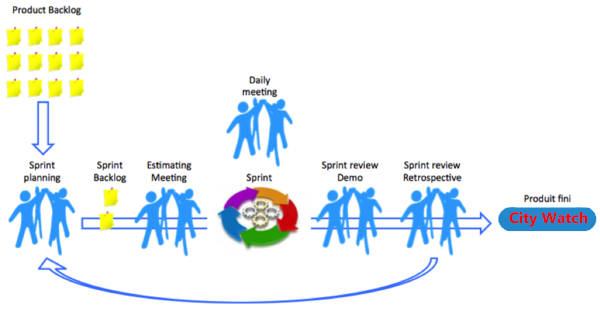
\includegraphics[width=\textwidth]{./figures/scrum-model.tex}
\begin{tikzpicture}

  \node[box]
    (sprints) {Sprints};
  \node[box, left=4em of sprints]
    (planning) {Planning \& System Architecture};
  \node[box, right=4em of sprints]
    (closure) {Closure};

  \draw[->,latex-,line width=0.1em] (5:6em) arc (5:85:6em) node[right=2em] {Wrap};
  \draw[->,latex-,line width=0.1em] (95:6em) node[left=2.5em] {Develop} arc (95:175:6em);
  \draw[->,latex-,line width=0.1em] (185:6em) arc (185:265:6em) node[left=2em] {Adjust};
  \draw[->,latex-,line width=0.1em] (275:6em) node[right=2.5em] {Review} arc (275:355:6em);

  \draw[->,latex-] (planning.west) -- +(-2em,0);
  \draw[->,-latex] (planning.east) to (sprints.west);
  \draw[->,-latex] (sprints.east) to (closure.west);
  \draw[->,-latex] (closure.east) -- +(2em,0);

\end{tikzpicture}
\caption[Méthode Scrum]{La méthode Génie Logiciel Scrum comme décrite par \textcite{Schwaber1995}.}
\captionsource{Daniel G. Siegel, Typical Development Processes of Free and Open Source Software Projects}
\label{fig:scrum-model}
\end{figure}

%\end{document}

\paragraph{Pourquoi SCRUM ?}
Scrum place l’humain au centre de la méthodologie. Le client intervient tout au long
du processus de création et l’équipe travaille en collaboration, et aussi parce que cette
méthode est idéale pour le cas d’une petite équipe et le fait d’avoir un grand projet réparti
entre cette équipe.
L’application de Scrum m’a permis de raccourcir les délais de production et d’avoir
un produit final qui correspond au plus près aux besoins du client.

\subsubsection{Répartition des rôles}
Chaque projet utilisant la méthode Scrum est monté autour d’une équipe auto-
organisée et multifonctionnelle : auto-organisée car il n’y a pas de chef d’équipe qui
décide les rôles de chacun, ou de la manière dont un problème est résolu, puisque ces
problématiques sont traitées par l’équipe dans son ensemble; et multifonctionnelle car
chaque membre de l’équipe forme une partie prenante dans le développement de
chaque fonctionnalité depuis l’idée jusqu’à l’implémentation finale.
Dans Scrum existe trois principaux rôles:
\begin{itemize}
 \item Le responsable produit (Product owner)
 \item Le Scrum Master
 \item le membre de l’équipe
\end{itemize}
\paragraph{Le responsable produit}
Il prend en charge de communiquer la
vision globale du produit à l’équipe. 
Il se voit représenter le client final, se met à sa place
et priorise ses besoins. Celui qui tient ce rôle est celui qui 
a le plus de visibilité, de responsabilité et d’autorité.
En effet, la méthode Scrum favorise l’auto-organisation de l'équipe.
\paragraph{Le Scrum Master}
Il joue le rôle du communiquant entre le responsable produit et
l’équipe. Il ne gère pas l’équipe, mais veille à éliminer tous les obstacles qui peuvent
empêcher l’équipe d’atteindre les objectifs fixés au cours d’un Sprint. En résumé, ce rôle
permet à l’équipe de rester créative et productive, tout en veillant à ce que les
réalisations soient visibles pour le responsable produit.
\paragraph{L'équipe}
Dans la méthode Scrum, l’équipe est responsable de la réalisation
opérationnelle des Sprints. L’équipe est généralement composée de personnes
multitâches. C’est toute l’équipe qui est responsable du résultat final de chaque sprint.
La manière dont sont exécutées les tâches est très libre mais cette liberté doit être
néanmoins cadrée par l’obligation de répondre aux objectifs du sprint.
\subsubsection{Durées estimées}
Pour montrer l’avancement durant une itération donnée, on a besoin de tracer le
Burndown Chart. Il s’agit d’un graphique simple qui montre le nombre d’heures restant
à effectuer pour finaliser le produit. 
\subsubsection{Modélisation UML}
\subsection{Backlog générale}
La première étape de la méthode Scrum consiste à préparer un carnet du produit
(Product Backlog) qui présente la liste des tâches à effectuer durant le développement
du projet qui sera répartie en des itérations. Le rôle du product-owner est important
dans cette phase de développement parce qu’il devra faire l’exercice de prioriser ses
demandes selon des critères respectant la mission et les objectifs de son produit. En
précisant la valeur de priorité, il estime l’impact et le retour sur investissement 
qu’aura chacun des items dans le carnet du produit.
Il y a donc effectivement eu un gros travail
d’échanges et discussions avec le client pour comprendre tout le cahier des charge
initial,C’est comme ça que le Backlog a été défini.

La figure~\ref{fig:product-backlog} présente une version simplifié du product
backlog décrit dans le tableau~\ref{tab:product-backlog}.
%\usepackage{dtklogos}
\usetikzlibrary{mindmap,shadows}
% Information boxes
\newcommand*{\info}[4][16.3]{%
  \node [ annotation, #3, scale=0.65, text width = #1em,
          inner sep = 2mm ] at (#2) {%
  \list{$\bullet$}{\topsep=0pt\itemsep=0pt\parsep=0pt
    \parskip=0pt\labelwidth=8pt\leftmargin=8pt
    \itemindent=0pt\labelsep=2pt}%
    #4
  \endlist
  };
}
\begin{tikzpicture}[every annotation/.style={draw, fill=white, font=\Large}]
    \renewcommand{\href}[2]{#2}

    \path[mindmap,
          concept color=black!40,
          text=white,
          every node/.style={
              concept,
              circular drop shadow,
              execute at begin node=\hskip0pt,
          },
          %grow cyclic,
          root/.style={
              concept color=black!40,
              fill=white, line width=1ex, text=black,
              font=\footnotesize\bfseries,
              text width=7em},
          level 1 concept/.append style={
              font=\normalsize\bfseries,
              sibling angle=50,
              text width=7.7em,
              level distance=12.5em,
              inner sep=0pt},
          level 2 concept/.append style={
              font=\footnotesize\bfseries,
              level distance=8em},
    ]

    node[root] {Platforme CityWatch} [clockwise from=0]
    child[concept color=blue!60] {
        node {Gestions des Rapports} [clockwise from=90]
        child { node (goForum) { Consultation } }
        child { node (goWiki) { Déclaration } }
    }
    child[concept color=blue] {
        node[concept] {Systeme de protection }
        [clockwise from=30]
        child { node[concept] (TeXnique)
            { Alert Secousses} }
        child { node[concept] (TeXweltQA)
            { Alert Doudannes} }
        child [faded] { node[concept] (TeXweltBlog)
            { Dedaction }}
    }
    child[concept color=green!40!black] {
        node[concept] {\href{http://texample.net/}{\TeX ample\\.net}}
        [clockwise from=310]
        child { node[concept] (TikZGalerie)
            {\href{http://texample.net/tikz/examples/}{TikZ-Galerie}} }
        child { node[concept] (TeXampleBlog)
            {\href{http://texample.net/weblog/}{Blog}} }
        child { node[concept] (Planet)
            {\href{http://texample.net/community/}{Planet}} }
    }
    child[concept color=red] {
        node[concept] (PGFPlots) {\href{http://pgfplots.net}{PGFPlots\\.net}}
        [clockwise from=270]
    }
    child[concept color=red!60!black] {
        node[concept] {\href{http://latex-community.org/}{\LaTeX-Community\\.org}}
        [counterclockwise from=100]
        child { node[concept] (LaTeXForum)
            {\href{http://latex-community.org/forum/}{Forum}}}
        child { node[concept] (LaTeXArtikel)
            {\href{http://latex-community.org/know-how}{Artikel-Archiv}} }
        child { node[concept] (LaTeXNews)
            {\href{http://latex-community.org/home/news}{News}} }
    }
    child[concept color=orange] {
        node[concept] (TeXdoc)
        {\href{http://texdoc.net/}{\TeX doc\\.net}}
        [clockwise from=100]
        child { node[concept] {\href{http://www.tex.ac.uk}{UK \TeX \\FAQ}}
        }}
    child[concept color=yellow!60!black] {
        node[concept] (Blogs) {Blogs} [clockwise from=139]
        child { node[concept] {\href{http://texblog.net/}{\TeX blog\\.net}}}
        child { node[concept] {\href{http://tikz.de/}{TikZ.de}} }
        child { node[concept] (Cookbook)
            {\href{http://latex-cookbook.net/}{\LaTeX-\\Cookbook\\.net}} }
    };
    %\info{goForum.north east}{above,anchor=west,xshift=1em}{%
    %  \item[] Seit 2008
    %  \item 68\,444 Beiträge
    %  \item 13\,715 Themen
    %  \item 5\,532 registrierte Nutzer
    %}
    %\info{LaTeXForum.north west}{above,anchor=south}{%
    %  \item[] Seit 2008
    %  \item 81\,991 Beiträge
    %  \item 21\,026 Themen
    %  \item 13\,354 registrierte Nutzer
    %}
    %\info[8]{LaTeXArtikel.west}{below,anchor=north east,xshift=3em,yshift=-2em}{%
    %  \item 115 Artikel
    %}
    %\info[11]{LaTeXNews.south west}{below,anchor=north}{%
    %  \item 240 Meldungen
    %}
    %\info[9]{TikZGalerie.south}{below,anchor=north}{%
    %  \item[] Seit 2006
    %  \item 172 Autoren
    %  \item 384 Beispiele
    %}
    %\info[15]{goWiki.south}{below,anchor=north,xshift=3em}{%
    %  \item 152 erklärte Konzepte, Befehle und Pakete
    %}
    %\info{TeXweltQA.south east}{above,anchor=north west}{%
    %  \item[] Seit 2013
    %  \item 1\,710 Fragen
    %  \item 2\,151 Antworten
    %  \item 479 registrierte Nutzer
    %}
    %\info[8]{TeXweltBlog.south}{below,anchor=north,xshift=2em}{%
    %  \item[] Seit 2013
    %  \item 14 Autoren
    %}
    %\info[9]{PGFPlots.south west}{anchor=north east,xshift=1em}{%
    %  \item 14 Autoren
    %  \item 59 Beispiele
    %}
    %\info[6]{Planet.west}{anchor=east}{%
    %  \item 46 Blogs
    %}
    %\info[14]{TeXnique.east}{anchor=west,xshift = 0.5em}{%
    %  \item[] 2015, aufgrund Idee mit französischen
    %          \TeX-Freunden nach der TUG Damstadt, experimentell
    %}
    %\info[16]{Cookbook.east}{anchor=south west}{%
    %  \item[] Ab 10/2015, soll ca. 100 Beispiele aus
    %          dem \LaTeX\ Cookbook zeigen, sowie
    %          Community-Rezepte
    %}
\end{tikzpicture}


\begin{center}
    \footnotesize
    \setlength\LTleft{-50pt}
\begin{longtable}{| l | p{3.5cm} | l | p{4.5cm} | p{4.5cm} | l |}
 \caption{Product Backlog}
 \label{tab:product-backlog} \\

 \hline
 \textbf{ID} & \textbf{Cas d'utilisations} & \textbf{En tant qu'} & \textbf{Je veux qu'} & \textbf{Pour} & \textbf{Priorité} \\ \hline
 \endhead

 \hline \multicolumn{6}{|r|}{{Continué en page suivante$\dotsc$}} \\ \hline
 \endfoot

 \hline \hline
 \endlastfoot

\hline
 1 & Gestion du Trajectoire & Utilisateur & Il soit possible de démarrer le tracking & Avoir un feedback dans l'application et sur le site web & 1 \\
   &                        & Utilisateur & Il soit possible d’arrêter le tracking & Avoir un feedback dans l’application & 1 \\ \hline
 2 & Gestion de Rapports    & Utilisateur & Il soit possible de choisir entre une variété de problèmes à déclarer depuis l’application & Avoir un feedback sur le site web & 1 \\
   &                        & Utilisateur & Il soit possible de choisir l’emplacement du problème à déclarer dans une carte & Avoir un feedback sur le site web & 1 \\
   &                        & Utilisateur & Il soit possible d’ajouter une description ou une image au problème & Avoir un feedback sur le site web & 2 \\ \hline
 3 & Consulter la carte     & Utilisateur & Il soit possible de consulter la carte depuis l’application & Voir la carte dans l’application & 2 \\ \hline
 4 & Compte                 & Utilisateur & Il soit possible de consulter le site web sans avoir un compte & Consulter le site web avec un minimum d’informations & 1 \\
   &                        & Utilisateur & Il soit possible de créer un compte & Avoir un compte personnel & 2 \\ \hline
 5 & Groupement des rapports& Utilisateur & Il est possible de voir les rapports en groupe lors d’un zoom out & Avoir une vision globale sur le nombre des rapports & 1 \\ \hline
 6 & Déclarer un rapport    & Utilisateur & Il est possible de déclarer un rapport à partir du site web & Avoir accès à une page rapport comme celle de l’application & 1 \\ \hline
\end{longtable}
\end{center}
\subsection{Conclusion}
L’itération 0 à permis de préparer le terrain pour une bonne entame de
développement. Mis à part la mise en place des environnement de travail et les
formations que nous avons suivi sur les technologies, cette itération a permis d’élaborer
le carnet de Plateforme CityWatch avec la collaboration du product owner et de fixer le
nombre des itérations et leur durée. Rappelons que l’itération 0 à durée trois jours,
du 20 février 2017 au 22 février 2017.
\newpage
\section{Itération 1}

\subsection{L'objectif du sprint}

Dans le but de définir le périmètre fonctionnel du Sprint 1 et faire
sa planification, tous les membres de l'équipe ont participé à un réunion
avec le Scrum Master et le Product Owner pour définir le backlog du sprint.\\

Une fois la première ébauche du Backlog est réalisée, le product owner peut découper
les spécifications de haut niveau vers des spécifications plus raffinées. Dès lors nous
passons à la planification d’une itération. Il est important de rappeler que les premières
spécifications du Backlog doivent être:
\begin{itemize}
 \item assez précise pour être estimée par l’équipe
 \item assez petite pour être développée et testée durant une itération
\end{itemize}
Ayant une bonne idée sur le produit ainsi que l’objectif à atteindre, l’équipe et le
product-owner peuvent passer à l’élaboration des itérations.
Dans notre projet ``Plateforme CityWatch'' la durée d’une Itération est fixée à trois
semaines (170h par itération). Dans ce chapitre nous décrivons le déroulement des deux
premières itérations. Une itération commence par sa planification et finit par être revue
avec ”Product-Owner”.

\subsubsection{Planification de l'itération 1}

La planification de l'itération représente une étape importante dans la vie de
l'itération parce que au cours du planification, on divise l'itération a plusieurs étapes
pour mieux atteindre le résultats attendu à la fin de l'itération.
Dans cette première itération on a décidé de diviser cette dernière en trois grandes
parties une partie consacrée pour la création de la base de donnée et la génération du
modèle, la deuxième partie est consacré pour la réalisation de la page d’accueil, et une
troisième partie qui répond aux besoins des autres tâches de cette itérations.

\subsubsection{But de la première itération}

Le but de cette itération est d'étudier notre Serveur ,de générer notre modèle,de réaliser
la page Web (dashboard) et développer les vues nécessaires pour permettre à l'utilisateur
de consulter la dernière position du véhicule selon les spécifications du Backlog.

\begin{center}
    \footnotesize
    \begin{longtable}{| p{1cm} | p{5cm} | p{7cm} | p{1cm} |}
        \caption{Taches à faire de la première itération}
        \label{tab:sprint1-backlog} \\

 \hline
 \textbf{Réf} & \textbf{Spécification} & \textbf{Description} & \textbf{Priorité} \\ \hline
 \endhead

 \hline \multicolumn{4}{|r|}{{Continué en page suivante$\dotsc$}} \\ \hline
 \endfoot

 \hline \hline
 \endlastfoot

\hline
1 & Présentation et Configuration SVN & Présenter SVN, installer le serveur SVN et créer les répertoires  & 1 \\ \hline
2 & Recherche sur les Services Web & Présenter les différentes Solutions des services web et choisir la meilleur solution & 1 \\ \hline
3 & Implémenter service Save Position & Enregistrement les coordonnées requis dans la base de données & 2 \\ \hline
4 & Implémenter la consommation du service Save Position & Coordonnées enregistrés instantané et continuellement dans la BD & 1 \\ \hline
5 & Recherche sur les spécifications de la plateforme Android & Présenter le modèle de développement Android et choisir le SDK optimale & 1 \\ \hline
6 & Création Application Template minimal & Application fonctionnel et intégration au SVN & 1 \\ \hline
7 & Implémenter service Get Last Position & Le serveur retourne les dernières coordonnées requis & 1 \\ \hline
8 & Rectification service Save Positon & Support multiple périphériques et enregistrer la date d'envoyé & 2 \\ \hline
9 & Rectification service Get Last Position & Retourné la position du périphérique et la date du dernier modification & 2 \\ \hline
10 & Affiche Multiple marqueurs & Afficher dernière position de chaque périphérique dans la carte & 2 \\ \hline
11 & Affiche état du périphérique & Afficher si le périphérique est en ligne ou hors ligne & 3 \\ \hline
\end{longtable}
\end{center}

\subsubsection{Estimation de la première itération}

Nous avons fixé la période d’une itération à 3 semaine. Dans
cette section, nous présentons une estimation du nombre d’heures pendant lesquelles
nous nous engageons à travailler.

\begin{table}[htbp]
    \centering
    \begin{tabular}{| c | c | c | c |}
\hline
\textbf{Membre} & \textbf{Nombre d'heures par jour} & \textbf{Nombre de jours présent} & \textbf{Total en heures} \\ \hline
\hline

Moez & 6 & 10 & 60\\ \hline
Rihab & 6 & 10 & 60 \\ \hline
\multicolumn{2}{c|}{} & \textbf{Total} & 120 \\ \cline{3-4}
    \end{tabular}
    \caption{Nombre d'heures de travail estimé de l'itération 1}
    \label{tab:sprint1-capacity}
\end{table}

\begin{center}
    \begin{longtable}{| l | l | l |}
        \caption{Nombre d'heures estimé pour la réalisation des taches}
        \label{tab:sprint1-estimation} \\

 \hline
 \textbf{Spécification} & \textbf{Membre} & \textbf{Heures} \\ \hline
 \endhead

 \hline \multicolumn{3}{|r|}{{Continué en page suivante$\dotsc$}} \\ \hline
 \endfoot

 \hline \hline
 \endlastfoot

\hline
Présentation et Configuration SVN & Rihab & 5 x 2 \\ \hline
Recherche sur les Services Web & Moez & 13 x 2 \\ \hline
Implémenter service Save Position & Moez & 5 \\ \hline
Implémenter la consommation du service Save Position & Rihab & 5 x 2 \\ \hline
Recherche sur les spécifications de la plateforme Android & Rihab & 13 x 2 \\ \hline
Création Application Template minimal & Rihab & 13 \\ \hline
Implémenter service Get Last Position & Moez & 5 \\ \hline
Rectification service Save Positon & Moez & 5 \\ \hline
Rectification service Get Last Position & Moez & 5 \\ \hline
Affiche Multiple marqueurs & Moez & 5 \\ \hline
Affiche état du périphérique & Rihab & 5 \\ \hline
\end{longtable}
\end{center}	

\subsection{Présentation des outils utilisés}

Le stage chez Djagora Academy nous a permis d'acquérir de nouvelles
compétences tant au nivrau relationnel que technique.Pour bien entamer la réalisation
de la plateforme 
``City Watch''nous avons suivi différentes
formations sur les outils et les technologies que nous venons de citer. 

\subsubsection{Apache Subversion}

Un logiciel de gestion de versions est un logiciel de gestion de configuration
permettant de stocker des informations pour une ou plusieurs ressources
informatiques permettant de récupérer toutes les versions intermédiaires des
ressources,vainsi que les différences entre les versions.

Apache Subversion (en abrégé SVN) est un logiciel de gestion de versions,
distribué sous licence Apache et BSD.
VisualSVN est un plug-in d’intégration de Subversion de qualité professionnelle.
Les principaux avantages de VisualSVN sont les suivants:

\begin{itemize}
    \item Fiabilité imbattable : Visual Studio ne s’arrêtera jamais ni ne
        s’arrêtera à cause de VisualSVN.
    \item Intégration transparente : VisualSVN gère automatiquement les fichiers
        ajoutés ou renommés et reflète ces opérations sur Subversion.
    \item Statut en temps réel : VisualSVN suit attentivement et affiche toutes
        les modifications apportées à votre copie de travail.
    \item Courbe d’apprentissage courte : VisualSVN utilise les boîtes de
        dialogue TortoiseSVN et fournit un assistant intelligent pour mettre
        vos sources sous Subversion.
\end{itemize}
VisualSVN Server vous permet d’installer et de gérer facilement un serveur
Subversion entièrement fonctionnel sur la plateforme Windows. Il est utile tant
pour les petites entreprises que pour les entreprises.

\subsubsection{Android}

Android est un système d'exploitation conçu en 2007 par la societé Android,
start-up racheté par Google . Android est Open Source, ca veut dire on peut lire
le code de ce logiciel le modifier et le redistribuer.

Les bases que nous utilisons:

\paragraph{IDE:}

C'est un logiciel dont son objectif est de faciliter le développement. Il est
toujours possible de développer une application sans IDE.
l'IDE est constitué d'outils dont au moins un éditeur de texte.
On utilisera dans notre projet l'IDE Android Studio, l'IDE privilège de Google.
Android Studio comporte l'auto-complétion la génération automatique  du code des
outils de compilation et débogage et plusieurs autres services qui permettent de
développer une application facilement et rapidement.

\paragraph{SDK:}

C’est une abréviation qui peut faire référence a Software Developpement Kit.
Les applications Android sont développés en JAVA. Un appareil Android ne
comprend pas le langage JAVA, il comprend une variante de JAVA adaptée pour lui.
On a recours ici SDK, c'est ensemble des outils permettant de développer dans
une cible particulière. Un SDK Android est alors un ensemble des outils qui
permettent de développer des application pour Android.

\paragraph{Activity:}

Un utilisateur habile d'Android remarque que lors de l'exploitation d'une
application Android qu'il est en train de naviguer entre des fenêtres et
l'application ne afficher qu'une seule fenêtre à la fois ces fenêtre la sont
des activités on peut différencier ces activité a travers leur interface
graphique ceci s'applique sur la plupart des application Android car il y a
des applications qui contiennent pas d'activités. Un première idée qui nous
frappe la tète c'est que une activité est un conteneur d'élément graphique qui
constitue un interface graphique. Alors que ne non une activité n'est pas
seulement une interface graphique mais elle va établir les liens entre
l'interface graphique et la logique programma tique de plus l'activité
contient des informations sur le statut actuel de l'application qui s'appelle le
contexte ce contexte permet de faire la liaison entre le système Android et les
autres activities de l'application.

\subparagraph{États d'activities:}

Le système Android met en place un système priorités entre application
par exemple l'utilisateur est en train de naviguer sur internet et écouter
de la musique il reçois un appel comme l'application qui gère les appel est
une application plus prioritaire elle prend la du navigateur et le lecteur
musique pour que l'utilisateur puisse répondre a son appel. Si une application
consomme trop de ressources et peut bloquer le fonctionnement du système Android,
Android arrêtera cette application. Et aussi comme expliqué précédemment
les activités sont gères a partir d'un système de pile d'activités .
D'où l'apparition de plus d'un état qui sont centré sur l'activité.

On peut différencier ces états par leur visibilité :
\begin{itemize}
 \item État Active
 \item État Paused
 \item État Stopped
\end{itemize}

\subparagraph{Cycle de vie d'une activité :}

Une activité n'a pas de contrôle sur son état.
Son état change suivant un cycle rythmique entre le système Android et les
AUTres application (un système quasi dépendant sur des priorités comme expliqué
précédemment) la figure~\ref{fig:android-activity} explique le cycle de vie
d'une activité. (Les états sont représenter comme des méthodes parce que lors de
la programmation ces états sont interroges par le nom de ces méthodes.\\
la figure~\ref{fig:android-activity} représente le cycle de vie d'une activité.

% Diagram of Android activity life cycle
% Author: Pavel Seda 
% Drawing part, node distance is 1.5 cm and every node
% is prefilled with white background
\begin{figure}[H]
 \centering
 \footnotesize

\begin{tikzpicture}[node distance=1.5cm,
    every node/.style={fill=white, font=\sffamily}, align=center]
  % Specification of nodes (position, etc.)
  \node (start)             [activityStarts]              {L'activité démarre};
  \node (onCreateBlock)     [process, below of=start]          {onCreate()};
  \node (onStartBlock)      [process, below of=onCreateBlock]   {onStart()};
  \node (onResumeBlock)     [process, below of=onStartBlock]   {onResume()};
  \node (activityRuns)      [activityRuns, below of=onResumeBlock]
                                                      {Activity is running};
  \node (onPauseBlock)      [process, below of=activityRuns, yshift=-1cm]
                                                                {onPause()};
  \node (onStopBlock)       [process, below of=onPauseBlock, yshift=-1cm]
                                                                 {onStop()};
  \node (onDestroyBlock)    [process, below of=onStopBlock, yshift=-1cm] 
                                                              {onDestroy()};
  \node (onRestartBlock)    [process, right of=onStartBlock, xshift=4cm]
                                                              {onRestart()};
  \node (ActivityEnds)      [startstop, left of=activityRuns, xshift=-4cm]
                                                        {Le processus est tué};
  \node (ActivityDestroyed) [startstop, below of=onDestroyBlock]
                                                    {l'activité est arrêtée};     
  % Specification of lines between nodes specified above
  % with aditional nodes for description 
  \draw[->]             (start) -- (onCreateBlock);
  \draw[->]     (onCreateBlock) -- (onStartBlock);
  \draw[->]      (onStartBlock) -- (onResumeBlock);
  \draw[->]     (onResumeBlock) -- (activityRuns);
  \draw[->]      (activityRuns) -- node[text width=4cm]
                                   {Une autre activité s'intercole devent notre activité} (onPauseBlock);
  \draw[->]      (onPauseBlock) -- node {Notre activité n'est plus visible}
                                   (onStopBlock);
  \draw[->]       (onStopBlock) -- node {L'activité est arrêtée par le système ou l'utilisateur} (onDestroyBlock);
  \draw[->]    (onRestartBlock) -- (onStartBlock);
  \draw[->]       (onStopBlock) -| node[yshift=1.25cm, text width=3cm]
                                   {L'activité revientsur le devant de la scène}
                                   (onRestartBlock);
  \draw[->]    (onDestroyBlock) -- (ActivityDestroyed);
  \draw[->]      (onPauseBlock) -| node(priorityXMemory)
                                   {Priorité élevée $\rightarrow$ plus mémoire}
                                   (ActivityEnds);
  \draw           (onStopBlock) -| (priorityXMemory);
  \draw[->]     (ActivityEnds)  |- node [yshift=-2cm, text width=3.1cm]
                                    {L'utilisateur retourne vers l'activité}
                                    (onCreateBlock);
  \draw[->] (onPauseBlock.east) -- ++(2.6,0) -- ++(0,2) -- ++(0,2) --
     node[xshift=1.2cm,yshift=-1.5cm, text width=2.5cm]
     {L'activité revient sur le devant de la scéne}(onResumeBlock.east);

  \end{tikzpicture}
  \caption{Diagramme de cycle de vie d'activite Android}
  \captionsource{Pavel Seda, \TeX example.net [Modifié]}{http://www.texample.net/tikz/examples/android/}
  \label{fig:android-activity}
\end{figure}


\subparagraph{Comment choisir le SDK optimale :}

Une SDK permet l'application de marcher sur la version Android visé
et les versions ultérieure il  a noté de prendre en considération le taux des
utilisateurs visé par cette application. Aussi il faut travailler avec une SDK
digne de confidence qui n'a pas de problème ou bug qui peuvent  bloquer ou arrêter
le fonctionnement de l'application le SDK choisi doit pouvoir supporter les
fonctionnalité offerte par l'application si on va utiliser une fonctionnalité
qui utilise les empreinte le SDK dont on a travailler l'application doit supporter
cette fonctionnalité lorsque le travail sur une application est en groupe il est
mieux que tous ce groupe utilise la même SDK pour éviter tous problème de
compatibilité et conflit entre versions de SDK  donc il faut choisir une SDK
qui est populaire en utilisation et qui est stable . Dans notre projet on va
utiliser SDK 23 qui vise la version Android 6.0 ayant un taux d'utilisateur
qui est 4.79 %
des utilisateur d'Android notons que cet SDK comporte
la fonctionnalité d'Android les plus récentes et qui est stable.

\subsubsection{Les Services Web}

Un service web est un protocole d'interface de communication et l'échange de
données entre applications et systèmes hétérogènes à distance en utilisant les
technologies Web.

Les variantes principales des services web sont:
\begin{itemize}
        \item \HTODO{SOAP/WSDL:}{add definition}
        \item \HTODO{REST:}{add definition}
\end{itemize}

\subsubsection{Lumen}

Pour le développement de backend du notre plateforme, la langue du programmation
PHP a été pré choisi. Mais, on avait la responsabilité de choisir les
bibliothèques et les frameworks. Pendant la 1\iere{} itération, le but était de
se familiariser avec la langue PHP. Donc, on a utilisé seulement les extensions
officiel du PHP includant PDO, $\dotsc$ . Dans l'itération suivante, on a étudié
les frameworks disponibles. A la fin, on a choisi le framework Lumen qui est
une version simplifié du Laravel pour le dévelopemment des API RESTful. Les
resons de choisir Lumen seront présentés dans le section du 2\ieme{} itération.

\subsection{Backlog du sprint}

Le sprint Backlog est un outil qui facilite la récupération des tâches et qui fait
la mise au point du travail tout en précisant les taches que contient chaque
user-story du Product Backlog.
Le Backlog agrée pour ce sprint est:

\TODO{sprint backlog}

\subsection{Mises des normes}

L'exigence de l'api RESTful est:
\begin{itemize}
    \item Performance: Le temps de réponse doit être en une durée raisonnable.
    \item Multi-Utilisateurs: Les positions des différents utilisateurs sont
        distinguables.
    \item Fiabilité: L'implémentation doit vérifier la structure des données
        reçus, la disponibilité des champs obligatoires et leurs formats.
    \item Portabilité: Le système doit support la différence en zone du temps
        et en internalisation, format de présentation des données géologique et
        sa précision.
\end{itemize}

Ces caractéristique ont étés adressés pendant l'implémentation du service web.

\subsubsection{Performance}

On a minimisé la dépendance en bibliothèques externes et extensions PHP.
De plus, Le nombre des requêtes SQL ont étés minimisés à une seule requêtes pour
chaque méthode du notre service web.

\subsubsection{Multi-Utilisateurs}

Les positions à enregistrer doivent contenus un id qui doit etre utiliser aussi
pour retirer la dernière position.
On a utilisé diffèrent identificateur pour chaque périphériques basé sur le MAC
du phone.

\subsubsection{Portabilité}

On a utilisé la format standardisée JSON pour le transfert de données ce qui
assure que la portabilité des représentations des différents types des données
(nombres, booléens, strings, $\dotsc$) indépendant du localisation.

Pour le représentation des dates dans le content du requêtes HTTP, on a utilisé
la format RFC3339 \cite{RFC3339} avec UTC comme la défaut zone du temps, ex:
\verb|2005-08-15T15:52:01|.

Pour les en-têtes du requêtes HTTP, la format de représentation des dates est
RFC1123 \cite{RFC1123}, ex: \verb|Mon, 15 Aug 2005 15:52:01 +0000|.

La format du présentation des positions géologique (latitude et longitude)
choisi est la même représentation des nombres en JSON avec une précision jusqu'à
14 chiffres après le virgule. Les valeurs envoyés doivent respecte l'intervalle
des diffèrent entités géologiques ($latitude \in [-90, 90]$,
$longitude \in [-180, 180]$)

\subsubsection{Fiabilité}

Pour assuré la fiabilité d'un service web, on doit vérifier la validité de
contenu reçu même si envoyé depuis un source de confiance avant de les
utiliser. La vérification inclue le test de disponibilité des entités
obligatoires et le test de leurs formats.

\TODO{add Position POST/GET apidoc}

\subsection{Modélisation UML}

\subsection{Évaluation suivant les normes mise}

\subsubsection{Page Web ``Dashboard''}

\TODO{sprint1 dashboard screenshot}

\subsubsection{Implementé la method POST}

Dans 1\ier{} phase, on a implémenté la méthode POST du ressource Position,

\TODO{RESTful API design describtion as http-api-design-en.pdf}

\subsection{Travail contribué}

\newpage
\section{Itération~2:~(~3/8/2017~-~3/28/2017~)}

\subsection{L'objectif du sprint}

La méthodologie Scrum a eu un impact positif sur les développeurs, du point de
vue social, elle a valorisé le travail en équipe, la solidarité, le respect et
la communication entre toutes les parties prenantes (client, développeurs,
\ldots). Elle a aussi changé leur vison sur le développement des logiciels.

L'objectif de cette itération est d'ajouter un système de gestion des rapport,
d'améliorer la qualité de service web de location et d'enrichir des
fonctionnalités du \textquote{Dashboard}.

\subsection{Planification de l'itération 2}

Au sein de la réunion de planification nous avons sélectionné les tâches à
réaliser au cours de cette itération tout en accord avec le \textquote{Product
Owner}.

\subsubsection{Backlog de l'itération}

\begin{center}
    \footnotesize
    \begin{longtable}{| p{1cm} | p{5cm} | p{7cm} | p{1cm} |}
        \caption{backlog de l'itération 2}
        \label{tab:sprint2-backlog} \\

        \hline
        \multicolumn{1}{|c}{\textbf{Réf}} &
        \multicolumn{1}{|c}{\textbf{Spécification}} &
        \multicolumn{1}{|c}{\textbf{Description}} &
        \multicolumn{1}{|c|}{\textbf{Priorité}} \\ \hline
        \endhead

        \hline \multicolumn{4}{|r|}{{Continué en page suivante$\dotsc$}} \\ \hline
        \endfoot

        \hline \hline
        \endlastfoot

        \hline
1 & Recherche sur les trajectoires & Comment présenter et enregistrer les trajectoire & 1 \\ \hline
2 & Affichage du trajet sur la carte & Visualizer le trajectoire d'un périphérique comme un ligne & 1 \\ \hline
3 & Implementer service d'enregsitrement des ralentisseurs & Enregistrer les données nécessaires pour représenter un ralentisseur & 1 \\ \hline
4 & Responsive design & IHM de l'applicaiont Android adaptable aux differents résolutions et rotations & 2 \\ \hline
5 & Implementer l'interface de déclaration un ralentisseur & Boutton rapport activé seulement si la localisation est active & 2 \\ \hline
6 & Filtrage des marqueurs dans la carte & Légende simplifiée permettant de choisir les types de données affichés dans la carte & 1 \\ \hline
7 & Implementer service de chargement de l'image & Charger, valider et enregistrer les images dans le serveur & 1 \\ \hline
8 & Implementer la fonctionnalité de déclaration des rapports & Formulaire avec validation et service d'enregistrement dans le serveur & 1 \\ \hline
9 & Recherche test unitaires & Comment améliorer la qualité du code et installation d'une solution des tests unitaires & 1 \\ \hline
10 & Recherche sur les frameworks PHP & Choisir le framework optimal pour notre platform et faire la migration & 2 \\ \hline
11 & Groupement de secousse sur la carte & Les marquers de secousses regroupés lors d'un zoom out sur la carte et séparer lors d'un zoom in & 3 \\ \hline
    \end{longtable}
\end{center}

\subsubsection{Estimation de la deuxième itération}

Comme l'itération précédant, Nous avons fixé la période de cette itération à 3
semaine.

\begin{table}[htbp]
    \centering
    \begin{tabular}{| c | c | c | c |}
        \hline
        \textbf{Membre} & \textbf{Nombre d'heures par jour} & \textbf{Nombre de jours présent} & \textbf{Total en heures} \\ \hline
        \hline
Moez & 8 & 18& 144\\ \hline
Rihab & 8 & 18 & 144 \\ \hline
\multicolumn{2}{c|}{} & \textbf{Total} & 288 \\ \cline{3-4}
    \end{tabular}
    \caption{Nombre d'heures de travail estimé de l'itération 2}
    \label{tab:sprint2-capacity}
\end{table}

\begin{center}
    \begin{longtable}{| l | l | l |}
        \caption{Nombre d'heures estimé pour la réalisation des taches}
        \label{tab:sprint2-estimation} \\

        \hline
        \multicolumn{1}{|c}{\textbf{Spécification}} &
        \multicolumn{1}{|c}{\textbf{Membre}} &
        \multicolumn{1}{|c|}{\textbf{Heures}} \\ \hline
        \endhead

        \hline \multicolumn{3}{|r|}{{Continué en page suivante$\dotsc$}} \\ \hline
        \endfoot

        \hline \hline
        \endlastfoot

        \hline
Recherche sur les trajectoires & Rihab & 5 x 2 \\ \hline
Affichage du trajet sur la carte & Moez & 13 x 2 \\ \hline
Implementer service d’enregsitrement des ralentisseurs & Moez & 5 \\ \hline
Responsive design & Rihab & 5 x 2 \\ \hline
Implementer l’interface de déclaration d'un ralentisseur & Rihab & 13 x 2 \\ \hline
Filtrage des marqueurs dans la carte & Rihab & 13 \\ \hline
Implementer service de chargement de l'image & Moez & 5 \\ \hline
Implementer la fonctionnalité de déclaration des rapports & Moez & 5 \\ \hline
Recherche test unitaires & Moez & 5 \\ \hline
Recherche sur les frameworks PHP & Moez & 5 \\ \hline
Groupement de secousse sur la carte & Rihab & 5 \\ \hline
    \end{longtable}
\end{center}

%\subsubsection{Évolution du travail}

\subsection{Présentation des outils utilisés}

\subsubsection{Lumen}

On a décidé de migrer vers un framework pour le développement du backend du
notre plateforme dans le but de simplifier et améliorer nos services web. Les
critères de choisir le framework étaient sa performance, sa stabilité et son
support de développement des api RESTful. Les 3 frameworks principales:
\begin{description}
    \item [Slim] Un macro framework performant avec support de développement
        des services web de premiere classe. Il manque le support pour
        développer des sites web classiques.
    \item [Symfony] Le framework PHP de référence. Il suivre une architecture
        modulaire et fournit une haute performance. Pour ajouter le support des
        services web, il nécessite l'ajoute et configurations des multiples des
        extensions.
    \item [Lumen] Une version minimal du framework Laravel pour le
        développement des services web. Étant basé sur Laravel, il profile d'un
        excellent support des extensions du troisième partie.
\end{description}

Lumen était choisi pour sa simplicité de configurer et de lancer et pour son
support de migrer vers Laravel en cas ou on aura besoin de supporter le
développement du site web classique ou autres types de développement.


%Pour le développement de backend du notre plateforme, la langue du
%programmation PHP a été pré choisi. Mais, on avait la responsabilité de choisir
%les bibliothèques et les frameworks. Pendant la 1\iere{} itération, le but
%était de se familiariser avec la langue PHP\@. Donc, on a utilisé seulement les
%extensions officiel du PHP incluant PDO, \ldots. Dans l'itération suivante, on
%a étudié les frameworks disponibles. A la fin, on a choisi le framework Lumen
%qui est une version simplifié du Laravel pour le développement des API
%\acrshort{RESTful}.

\subsection{Mises des normes}

Outres que les critères de la premiere itération, les nouveaux critères à
respecter pour cette itération sont:

\paragraph{Qualité d trajectoire}
Le trajectoire doit être aligné sur le trajet avec bonne précision. Et le
nombre des positions nécessaire pour tracer le trajectoire doivent être le
minimum le plus possible.

\paragraph{Architecture modulaire}
Architecture de backend doit être modulaire: On doit changer notre code
procédurale par un code orienté objet et minimiser la duplication du code et
séparer le code des models et le code des contrôleurs.

\paragraph{IHM de la page Dashboard Responsive}
Affiche claire et responsive des marqueurs dans la carte meme si le nombre est
très élevé.

\subsection{Modélisation UML}

\begin{figure}[htbp]
    \centering
    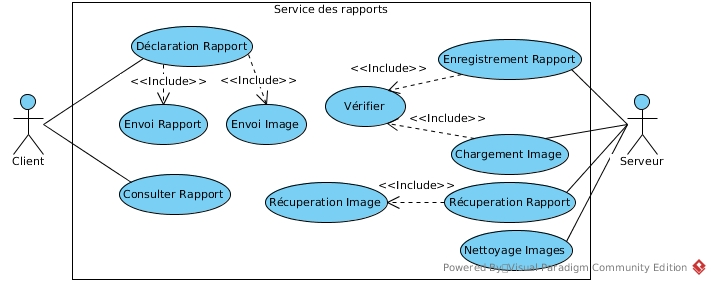
\includegraphics[width=1\textwidth]{sprint2-webservices-report-usecase}
    \caption{Diagramme de case d'utilisation du services Rapports en itération 2}
\end{figure}

\begin{figure}[htbp]
    \centering
    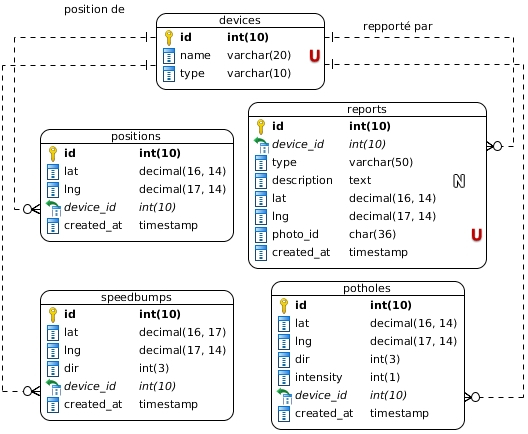
\includegraphics[width=1\textwidth]{sprint2-webservices-database}
    \caption{Diagramme entité-association du service Position en itération 2}
\end{figure}

\begin{figure}[htbp]
    \centering
    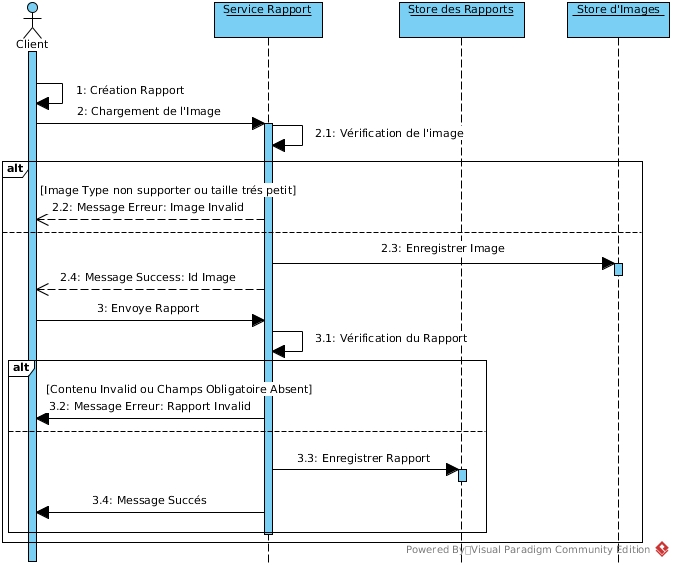
\includegraphics[width=1\textwidth]{sprint2-webservices-report-post-sequence}
    \caption{Diagramme de séquence du services Post Rapports en itération 2}
\end{figure}

\begin{figure}[htbp]
    \centering
    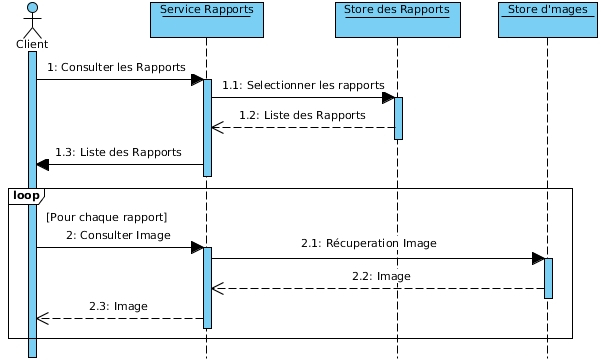
\includegraphics[width=1\textwidth]{sprint2-webservices-report-get-sequence}
    \caption{Diagramme de séquence du services Get Rapports en itération 2}
\end{figure}

\subsection{Évaluation suivant les normes mise}

\TODO{EVALUATION}

\subsection{Contributions}

Au cours de l'itération avec l'augment des fonctionnalités ajoutées au
Dashboard, le code JavaScript devenu complexe, dupliqué et difficile à détecter
les bugs. On a décidé de réécrire le code avec une architecture modulaire et
plus moderne.

L'utilisation de la version ECMAScript 6 du JavaScript nous a fourni les
techniques de base nécessaires comme POO, Template Strings, paramètres par
défaut, nouvelles variantes de la boucle For et support de la programmation
asynchrone.

\TODO{add class diagram}

La nouvelle architecture a consisté de:
\begin{itemize}
    \item Une classe \verb|Map| contenu tout le logique métier d'initialiser et
        afficher la carte, registre et filtrer des différents types de données
        et traiter les différents évènements d'interaction humaine machine.
    \item Une classe abstract \verb|Layer| contenu tout le logique relié à
        chaque types des données à visualiser dans la map (téléchargement
        continuellement les données, génération les marqueurs ou zones, mise à
        jour des données, définition des filtrages supportés et les
        informations additionnelles à afficher). Le code commun entre différents
        layers est implémenté dans cette classe abstract.
    \item Une classe pour chaque type de données à visualiser (trajectoire,
        ralentisseurs, secousses, \ldots) qui hérite du class \verb|Layer|. La
        plupart du temps, on a juste besoin de définir l'URL du resource, la
        listes des icons et des filtrages possibles.
    \item Un espace de noms \verb|Config| contenu les variables de
        configuration.
\end{itemize}

\subsection{Revue de cette itération}

\subsubsection{Produit de l'itération}

A la fin de l'itération 2,nous détaillons les différentes spécifications qui
caractérisent et implémenté le système de gestion des rapport.

\paragraph{Page \textquote{Rapport}}

Dans cette page, nous donne la main à l'utilisateur pour faire un petit rapport
comme expliqué dans la figure~\ref{fig:sprint2-rapport-screenshot1}. Cette page
permet à l'utilisateur d'envoyer son rapport au serveur pour l'enregistrer.
La position du rapport est détecté automatique à travers l'api JavaScript
standard Location. On donne la main à l'utilisateur pour changer la location
manuellement en glissant le marqueur ou en changer les inputs. Le chargement de
l'image est obligatoire.

\TODO{Cette obligation était éliminer en review}

L'envoie du rapport est éxecuté en deux phases:
\begin{enumerate}
    \item Chargement de l'image au serveur. Si le type et le taille de l'image
        est valide, le serveur retourne un id unique (UUID) de l'image.
    \item Envoie du rapport au serveur. Les informations envoyées sont: type du
        rapport, id image, commentaire (optionnel) et les coordonnées.
\end{enumerate}

\begin{figure}[htbp]
    \centering
    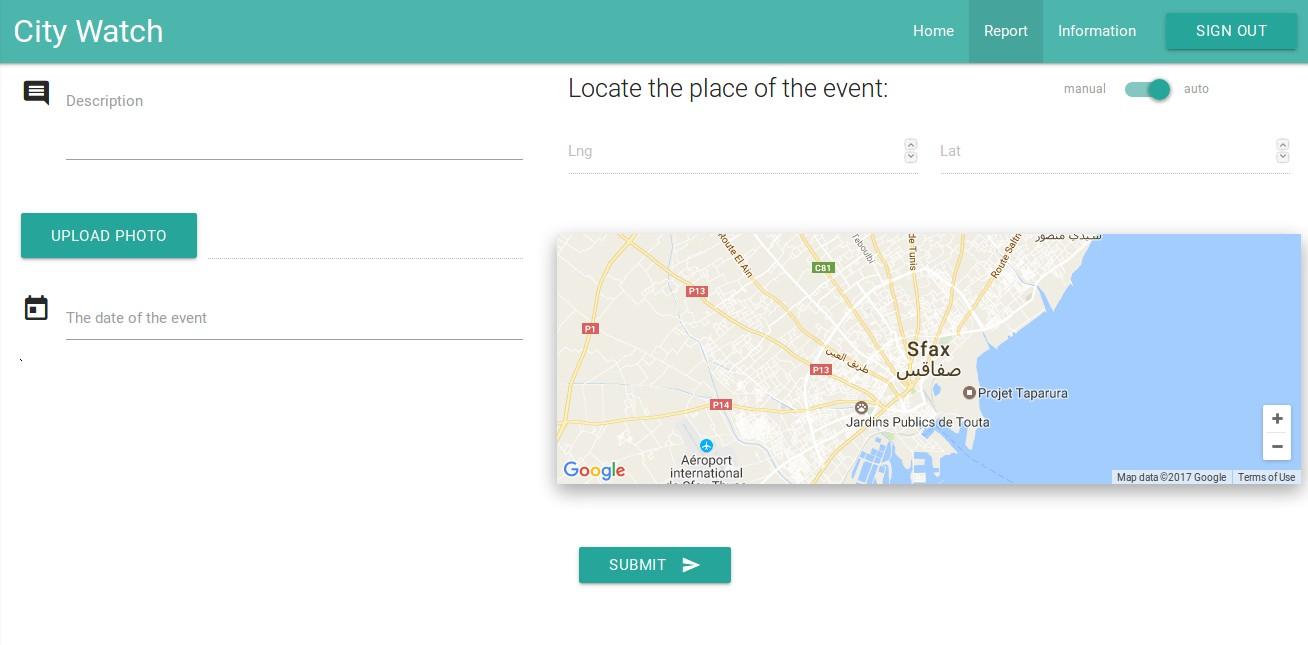
\includegraphics[width=0.7\textwidth]{sprint2-rapport-screenshot1}
    \caption{Page Rapport}
    \label{fig:sprint2-rapport-screenshot1}
\end{figure}

\paragraph{Page \textquote{Dashboard}}
L'utilitaire de regroupement de marqueurs vous aide à gérer plusieurs marqueurs
à différents niveaux de zoom. Précisément, les marqueurs sont en fait des
éléments à ce stade et ne deviennent réellement des marqueurs qu'après leur
rendu. Par souci de clarté, nous ne parlerons que de marqueurs dans ce
document.

Lorsqu'un utilisateur affiche la carte à un niveau de zoom élevé comme montre
la figure~\ref{fig:sprint2-dashboard-screenshot1}, les différents marqueurs
s'affichent sur la carte. Lorsqu'il effectue un zoom arrière comme montre la
figure~\ref{fig:sprint2-dashboard-screenshot2}, les marqueurs se regroupent
pour faciliter la consultation de la carte.

\begin{figure}[htbp]
    \begin{subfigure}{.5\textwidth}
        \centering
        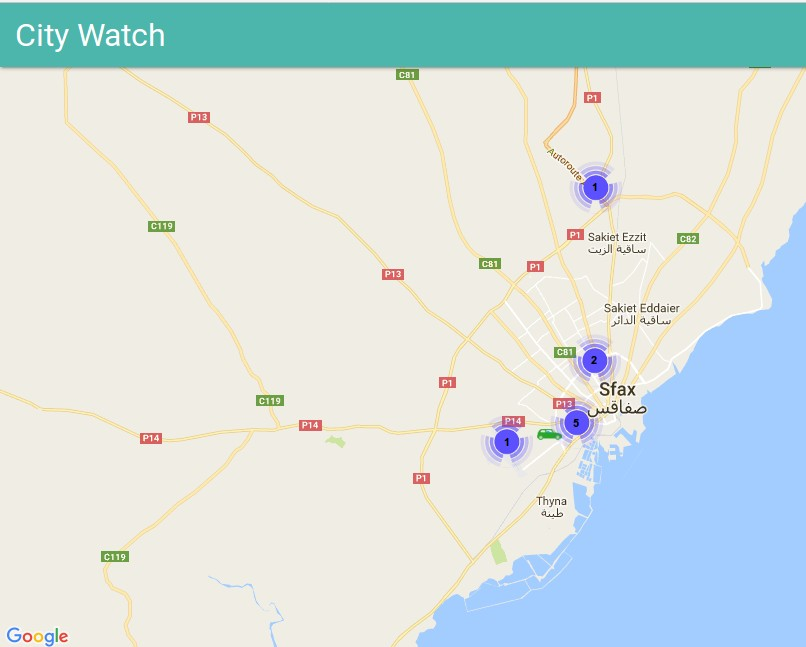
\includegraphics[width=.8\linewidth]{sprint2-dashboard-screenshot1}
        \caption{Groupement activé en un zoom bas}
        \label{fig:sprint2-dashboard-screenshot1}
    \end{subfigure}
    \begin{subfigure}{.5\textwidth}
        \centering
        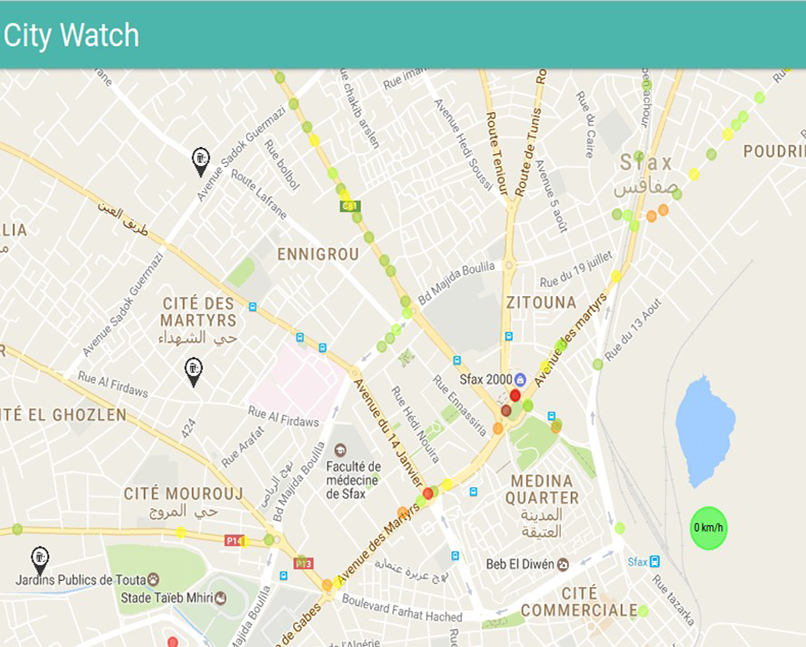
\includegraphics[width=.93\linewidth]{sprint2-dashboard-screenshot2}
        \caption{Groupement désactivé en zoom haut}
        \label{fig:sprint2-dashboard-screenshot2}
    \end{subfigure}
    \caption{Groupement des marqueurs des secousses en différents niveaux du zoom}
\end{figure}
\clearpage

\paragraph{Application Mobile \textquote{CityWatch}}

Dans notre application, l'utilisateur doit s'inscrit pour accéder à
l'application.

\TODO{Description}

\begin{figure}[htbp]
    \begin{subfigure}{.5\textwidth}
    \centering
  \centering
  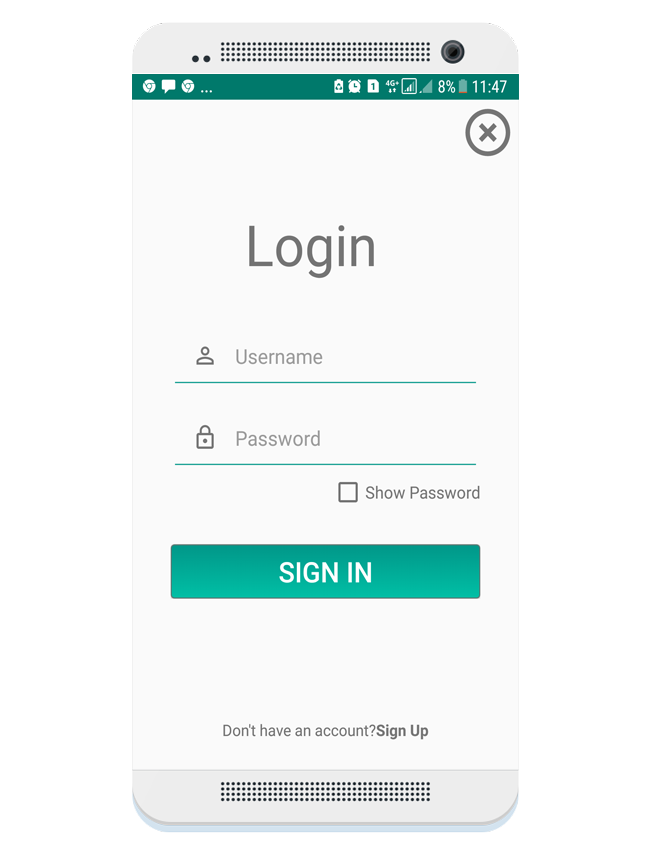
\includegraphics[width=.7\linewidth]{sprint2-android-screenshot1}
  \caption{Activity login}
  \label{fig:sprint2-android-screenshot1}
\end{subfigure}
\begin{subfigure}{.5\textwidth}
    \centering
  \centering
  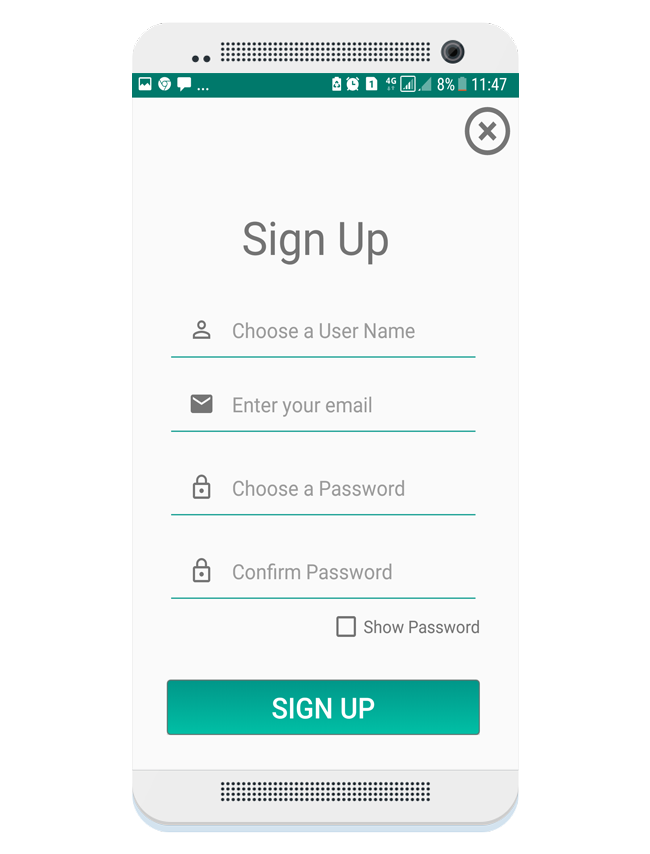
\includegraphics[width=.7\linewidth]{sprint2-android-screenshot2}
  \caption{Activity sing up}
  \label{fig:sprint2-android-screenshot2}
\end{subfigure}
\caption{Interface de l'application au deuxième itération}
\end{figure}

\subsubsection{Avis du Product Owner}

A la fin de cette première itération, nous avons présenté au \textquote{Product
Owner} le produit obtenu. Le \textquote{Product Owner} a exprimé sa
satisfaction du travail.

\subsubsection{Graphique d'avancement de l'itération}

\usetikzlibrary{plotmarks}

\begin{figure}
\centering
\begin{tikzpicture}[y=.1cm, x=.7cm,font=\sffamily]
\begin{axis}[
xlabel=$Jours$,
ylabel=$Heures\ restantes$,
grid=both,
grid style={line width=.1pt, draw=gray!10},
width=0.9\textwidth,
height=10cm,
%major grid style={line width=.2pt,draw=gray!50},
]
\addplot[color=black,mark=*] coordinates {
        (0,144)
        (18,0)
    };
    \addlegendentry{Temps Idéal}

    \addplot[mark=*,red] plot coordinates {
        (0, 144)
        (1, 138)
        (2, 130)
        (3, 125)
        (4, 122)
        (5, 115)
        (6, 111)
        (7, 108)
        (8, 100)
        (9, 92)
        (10, 88)
        (11, 88)
        (12, 85)
        (13, 80)
        (14, 72)
        (15, 60)
        (16, 55)
        (17, 48)
        (18, 40)
       
    };
    \addlegendentry{Rihab}
      \addplot[mark=*,cyan] plot coordinates {
        (0, 144)
        (1, 130)
        (2, 125)
        (3, 120)
        (4, 110)
        (5, 100)
        (6, 100)
        (7, 100)
        (8, 98)
        (9, 90)
        (10, 82)
        (11, 73)
        (12, 72)
        (13, 60)
        (14, 49)
        (15, 41)
        (16, 35)
        (17, 30)
        (18, 22)
       
    };
    \addlegendentry{Moez}
\end{axis}
\end{tikzpicture}
\caption{Graphique d'avancement - Itération 2}
\end{figure}


\newpage
\section{Itération 3: ( 4/3/2017 - 4/28/2017 )}

\subsection{L'objectif du sprint}
Le Product Owner nous a demandé d’améliorer le chargement de l'image 
dans le serveur de telle sorte que la qualité d'image reste la même..
Donc, dans cette itération, nous allons tenir compte des attentes du Product Owner. Nous allons
modifier le critère de chargement, En plus nous allons implémenter une méthode
permettant de maintenir la qualité.

\subsubsection{Planification de l'itération 3}

\subsubsection{Préparation de la liste des tâches}

Le but de cette itération est d'ajouter un système de gestion des rapport et d'améliorer
la qualité.

\begin{center}
    \footnotesize
    \begin{longtable}{| p{1cm} | p{5cm} | p{7cm} | p{1cm} |}
        \caption{Taches à faire de la troisième itération}
        \label{tab:sprint3-backlog} \\

 \hline
 \multicolumn{1}{|c}{\textbf{Réf}} &
 \multicolumn{1}{|c}{\textbf{Spécification}} &
 \multicolumn{1}{|c}{\textbf{Description}} &
 \multicolumn{1}{|c|}{\textbf{Priorité}} \\ \hline
 \endhead

 \hline \multicolumn{4}{|r|}{{Continué en page suivante$\dotsc$}} \\ \hline
 \endfoot

 \hline \hline
 \endlastfoot

\hline
1 & Web View & Implémenté la méthode qui affiche les pages ``Dashboard et Rapport'' chacun a un bouton spécifié   & 1 \\ \hline
2 & Authentification Restful  & Ajouter l'authentification dans le serveur pour assurer la sécurité   & 1 \\ \hline
3 & landing page & créer une nouvel page Web  & 3\\ \hline
4 & Realisation de la BD liée au comptes utilisateur& Base de données accecible depuis l'application et le web& 2 \\ \hline
5 & Post réseau & Methode POST Restful & 1 \\ \hline
6 & GET réseau & Methode GET Restful & 1 \\ \hline
7 & Post vitesse & Methode vitesse & 1 \\ \hline
8 & Get vitesse & Methode GET & 1 \\ \hline
9 & Responsive & Responsive design coter android & 3 \\ \hline
10 & IHM & l'ajout des boutons radio pour distinguer (pieton / voiture)(android) & 3 \\ \hline
11 & Recherche Bissnes intelligence & BI & 2 \\ \hline
12 & Implantation des BD au BI & données accessible en BI & 2\\ \hline
13 & création Logo &Ajouter Logo dans l'application & 3 \\ \hline
14 & Comercialisation & ...& ...\\ \hline
15 & Rectification update manager &..... & 1 \\ \hline



\end{longtable}
\end{center}

\subsubsection{Estimation de la deuxième itération}
\begin{table}[htbp]
    \centering
    \begin{tabular}{| c | c | c | c |}
\hline
\textbf{Membre} & \textbf{Nombre d'heures par jour} & \textbf{Nombre de jours présent} & \textbf{Total en heures} \\ \hline
\hline

Moez & 8 & 15 & 120\\ \hline
Rihab & 8 & 15 & 120 \\ \hline
\multicolumn{2}{c|}{} & \textbf{Total} & 240 \\ \cline{3-4}
    \end{tabular}
    \caption{Nombre d'heures de travail estimé de l'itération 3}
    \label{tab:sprint3-capacity}
\end{table}

\begin{center}
    \begin{longtable}{| l | l | l |}
        \caption{Nombre d'heures estimé pour la réalisation des taches}
        \label{tab:sprint3-estimation} \\

 \hline
 \multicolumn{1}{|c}{\textbf{Spécification}} &
 \multicolumn{1}{|c}{\textbf{Membre}} &
 \multicolumn{1}{|c|}{\textbf{Heures}} \\ \hline
 \endhead

 \hline \multicolumn{3}{|r|}{{Continué en page suivante$\dotsc$}} \\ \hline
 \endfoot

 \hline \hline
 \endlastfoot

\hline
Web view& Rihab & 5 x 2 \\ \hline
Authentification Restful& Rihab & 5 x 2 \\ \hline
landing page& Rihab & 5 x 2 \\ \hline
Realisation de la BD liée au comptes utilisateur& Rihab & 5 x 2 \\ \hline
Post réseau& Rihab & 5 x 2 \\ \hline
GET réseau& Rihab & 5 x 2 \\ \hline
Post vitesse& Rihab & 5 x 2 \\ \hline
Get vitesse& Rihab & 5 x 2 \\ \hline
Responsive& Rihab & 5 x 2 \\ \hline
IHM & Rihab & 5 x 2 \\ \hline
Recherche Bissnes intelligence& Rihab & 5 x 2 \\ \hline
Implantation des BD au BI& Rihab & 5 x 2 \\ \hline
création Logo& Rihab & 5 x 2 \\ \hline
Comercialisation& Rihab & 5 x 2 \\ \hline
Rectification update manager& Rihab & 5 x 2 \\ \hline
\end{longtable}
\end{center}

\subsection{Backlog du sprint}

\subsection{Mises des normes}

\subsection{Modélisation UML}

\subsection{Évaluation suivant les normes mise}

\subsection{Travail contribué}


%%%% INCLUDE CHAPTERS

\clearpage
\renewcommand{\sectionmark}[1]{\markright{\thesection\ \ --\ \ #1}}
%\appendix
\section{Annexe}
\pagebreak

\subsection{Documentation des Services Web d'itération 1}

\subsubsection{Service Post Position}
\label{appendix:sprint1-position-post-doc}

\textbf{POST} \ \texttt{/positions/\textit{:id}}

\begin{table}[htbp]
    \centering
    \caption*{Paramètres Service Post Position}
    \begin{tabular}{llll}
        \toprule
        \multicolumn{1}{c}{\textbf{Élément}} &
        \multicolumn{1}{c}{\textbf{Obligation}} &
        \multicolumn{1}{c}{\textbf{Type}} &
        \multicolumn{1}{c}{\textbf{Description}} \\
        \midrule
        \verb|:id| & obligatoire & string & identificateur du périphérique \\
        \verb|lat| & obligatoire & nombre [-90, 90] & latitude de la position \\
        \verb|lng| & obligatoire & nombre [-180, 180] & longitude de la position \\
        \verb|last_modified| & optionnel & string (RFC3339) & date du capture de la position \\
        \bottomrule
    \end{tabular}
\end{table}

\subparagraph*{Réponse Codes}
\begin{description}
    \item[\texttt{204 No Content}] Position était crée ou mette à jour avec succès.
    \item[\texttt{400 Bad Request}] Le contenu JSON n'est pas valide.
    \item[\texttt{422 Unprocessable Entity}] Entité obligatoire absente ou format d'une entité est invalide.
\end{description}

\subparagraph*{Entités de réponse}

n/a

\begin{listing}
    \caption*{Démonstration Service Post Position}
    \begin{minted}[label={Requéte}]{bash}
curl -i -X POST http://localhost/positions/1 \
     -d '{"lat": 10.71979600000000,
          "lat": "34.72563400000000",
          "last_modified": "2017-03-27 10:34:01"}' \
     -H 'Content-Type: application/json'
\end{minted}
\begin{minted}[label={Réponse en Succés}]{http}
HTTP/1.1 200 Success
Content-Type: application/json

{
    "success": true
}
\end{minted}
\end{listing}

\clearpage
\subsubsection{Service Get Position}
\label{appendix:sprint1-position-get-doc}

\textbf{GET} \ \texttt{/positions/\textit{:id}}

\begin{table}[htbp]
    \centering
    \caption*{Paramètres Service Get Position}
    \begin{tabular}{llll}
        \toprule
        \multicolumn{1}{c}{\textbf{Élément}} &
        \multicolumn{1}{c}{\textbf{Obligation}} &
        \multicolumn{1}{c}{\textbf{Type}} &
        \multicolumn{1}{c}{\textbf{Description}} \\
        \midrule
        \verb|:id| & obligatoire & string & identificateur du périphérique \\
        \bottomrule
    \end{tabular}
\end{table}

\begin{table}[htbp]
    \centering
    \caption*{Entités du réponse du Service Post Position}
    \begin{tabular}{lll}
        \toprule
        \multicolumn{1}{c}{\textbf{Élément}} &
        \multicolumn{1}{c}{\textbf{Type}} &
        \multicolumn{1}{c}{\textbf{Description}} \\
        \midrule
        \verb|lat| & nombre [-90, 90] & latitude de la position \\
        \verb|lng| & nombre [-180, 180] & longitude de la position \\
        \bottomrule
    \end{tabular}
\end{table}

\begin{table}[htbp]
    \centering
    \caption*{En-tête Réponse Service Get Position}
    \begin{tabular}{llll}
        \toprule
        \multicolumn{1}{c}{\textbf{En-tête}} &
        \multicolumn{1}{c}{\textbf{Type}} &
        \multicolumn{1}{c}{\textbf{Description}} \\
        \midrule
        \verb|Last-Modified| & string (RFC1123) & Date du dernier modification du position \\
        \bottomrule
    \end{tabular}
\end{table}

\subparagraph*{Réponse Codes}
\begin{description}
    \item[\texttt{200 Success}] Dernière position du périphérique spécifié retournée.
    \item[\texttt{404 Not Found}] Aucune position trouvée pour le périphérique spécifié.
\end{description}

\begin{listing}
    \caption*{Démonstration Service Get Position}
    \begin{minted}[label={Requéte}]{bash}
curl -i http://localhost/api/v1/positions/1
\end{minted}
\begin{minted}[label={Réponse en Succés}]{http}
HTTP/1.1 200 OK
Content-Type: application/json
Last-Modified: Wed, 17 May 2017 14:51:00 GMT

{
    "lng": "10.71989600000000",
    "lat": "34.72526400000000"
}
\end{minted}
\end{listing}

\clearpage
\subsection{Documentation des Services Web d'itération 2}

\TODO{doc}

\clearpage
\subsection{Documentation des Services Web d'itération 3}

\TODO{doc}

\clearpage
\section{Annexe}

\subsection{Evolution du qualité du code}

\TODO{use Hits by Response Code chart from server state to show code quality improvement}


% APPENDEX A, B, ...

\clearpage
\fancypagestyle{plain}{
    \fancyhf{}
    \rfoot{\thepage}
    \renewcommand{\headrulewidth}{0pt}
    \renewcommand{\footrulewidth}{0pt}
}
\pagestyle{plain}

% \printglossary[type=\acronymtype]
%\addcontentsline{toc}{section}{Glossaire des Acronymes}
\glossarystyle{altlistgroup}
\glsaddall
\printglossaries

\clearpage
\nocite{*}
\printbibheading
\printbibliography[type=book,heading=subbibliography,title={Livres}]
\printbibliography[nottype=book,heading=subbibliography,title={Autres Sources}]

% \listoftodos % TODO FIXME list

\end{document}
